\documentclass[11pt,mathserif]{beamer} %You need this at the top to declare that you're using Beamer 

%----------------------------------------------------------------------------------------------------------------------------------------------%
%%%%%%%%% Before we start putting the presentation together, need to declare formating and packages %%%%

%%%%%%%%%%%%%%% Standard packages%%%%%%%%%%%%%%%
\usepackage{algorithm,algorithmic}  %2 packages for making nice looking algorithms
\usepackage{amsmath,mathtools} %Standard math commands (like vectors, symbols, etc.)
\usepackage{epsfig,epstopdf} %You need these if you have .eps vector graphics (recommend if possible)
%\usepackage{tikz} %Sometimes you may want to use Tikz to make figures (but its pretty complicated)
\usepackage{media9} %If you want to include movies (like in my earlier presentation) you'll need this package
%%% Below are packages commonly used for making figures
\usepackage{subfigure,MnSymbol,pdfpages}
\usepackage{graphicx,color,colortbl}
\usepackage{bm,amsfonts,graphics}

\usepackage{listings} %You won't need this unless youre displaying source code - I DONT RECOMMEND YOU DO THIS YET



%%%%%%%%%%%%%%% Commands for making the ACL slide format %%%%%%%%%%%%%%%%%
\setbeamercolor{block title}{bg=blue!55,fg=black}%bg=background, fg= foreground
\setbeamercolor{block body}{bg=blue!20,fg=black}%bg=background, fg= foreground
\renewcommand{\vec}[1]{\mathbf{#1}} %Changes the ``vec'' command for vectors to bold font rather than arrows overhead
\usepackage{amsmath}
\usepackage{mathtools}
\usepackage{tikz}
%\usepackage{movie15}
\usepackage{algorithm} % must read after hyperref
\usepackage{algorithmic}
\usepackage{subfigure,MnSymbol}
\usepackage{graphicx,color,colortbl}
%\usepackage[footnotesize,bf]{caption}
\usepackage{bm,amsfonts,graphics}
\usepackage{tikz,tkz-graph,tkz-arith,tkz-berge}
\usetikzlibrary{arrows,shapes,positioning}

\graphicspath{{./}{figures/}}
\usepackage{multicol}

\newtheorem{thm}{Theorem}
\newtheorem{lem}{Lemma}
\newtheorem{prop}{Proposition}
\newtheorem{rem}{Remark}

\newcommand{\jcols}[4]{
\begin{columns}[T]\begin{column}[T]{#3\textwidth} #1 \end{column}
\begin{column}[T]{#4\textwidth} #2 \end{column}
\end{columns}}

\newcommand{\jcolsb}[4]
{\begin{columns}[b]
\begin{column}{#3\textwidth} #1 \vspace{0pt}
\end{column}
\begin{column}{#4\textwidth} #2 \vspace{0pt}
\end{column}
\end{columns}}

\newcommand{\jcolsc}[4]
{\begin{columns}[c]
\begin{column}{#3\textwidth} #1 \vspace{0pt}
\end{column}
\begin{column}{#4\textwidth} #2 \vspace{0pt}
\end{column}
\end{columns}}
\mode<presentation>
{
	\usetheme{ACL}
        \setbeamercovered{transparent=0}
}

\makeatletter
\newdimen\labelwidthi
\newdimen\labelwidthii
\newdimen\labelwidthiii
\newdimen\labelwidthiv
\def\normal@labelsep{0.2em}
\labelsep\normal@labelsep
\settowidth{\labelwidthi}{iii}
\settowidth{\labelwidthii}{ii}
\settowidth{\labelwidthiii}{iii}
%\settowidth{\labelwidthiv}{i}
\setlength\leftmargini{0pt}
\setlength\leftmarginii{1.5ex}
\setlength\leftmarginiii{1.5ex}

\leftmargini\labelwidthi    \advance\leftmargini\labelsep
\leftmarginii\labelwidthii  \advance\leftmarginii\labelsep
\leftmarginii\labelwidthiii \advance\leftmarginiii\labelsep

%\leftmarginii\labelwidthiv  \advance\leftmarginiv\labelsep
%\def\setleftmargin#1#2{\settowidth{\@tempdima}{#2}\labelsep\normal@labelsep
%  \csname labelwidth#1\endcsname\@tempdima
%  \@tempdimb\@tempdima \advance\@tempdimb\labelsep
%  \csname leftmargin#1\endcsname\@tempdimb}
%\def\@listI{\leftmargin\leftmargini
%  \labelwidth\labelwidthi \labelsep\normal@labelsep
%  \topsep \z@ \partopsep\z@ \parsep\z@ \itemsep\z@
%  \listparindent 1em}
%\def\@listii{\leftmargin\leftmarginii
%  \labelwidth\labelwidthii \labelsep\normal@labelsep
%  \topsep\z@ \partopsep\z@ \parsep\z@ \itemsep\z@
%  \listparindent 1em}
%\def\@listiii{\leftmargin\leftmarginiii
%  \labelwidth\labelwidthiii \labelsep\normal@labelsep
%  \topsep\z@ \partopsep\z@ \parsep\z@ \itemsep\z@
%  \listparindent 1em}
%\def\@listiv{\leftmargin\leftmarginiv
%  \labelwidth\labelwidthiv \labelsep\normal@labelsep
%  \topsep\z@ \partopsep\z@ \parsep\z@ \itemsep\z@
%  \listparindent 1em}
%\let\@listi\@listI
%\@listi
\makeatother

\logo{

\includegraphics[height = 0.6cm,trim=0 50 0 0,clip]{AO-logo-high_color-top-MIT}

\includegraphics[height = 0.5cm,trim=0 0 0 0,clip]{ACL_logo}
}

\setbeamerfont{frametitle}{size=\large,series=\bfseries}
%\setbeamertemplate{frametitle}[default][center]
\setbeamerfont{title}{size=\large,series=\bfseries}
\setbeamerfont{framesubtitle}{series=\mdseries,size=\large}
\graphicspath{{./}{figures/}}
\usepackage[square, numbers, comma]{natbib}	% use Natbib for author-name
									% citations. In a presentation,
									% this is more legible than pure
									% numbers, like [21]. Google
									% "natbib" for more information.
									% Instead of "\cite{abc}", use
									% "\citep{abc}" or "\citet{abc}"
\bibliographystyle{plainnat}		% Natbib specific
%\bibpunct{(}{)}{,}{a}{}{,}			% Natbib specific

\definecolor{Maroon}{RGB}{112,0,0}
\definecolor{Crimson}{RGB}{200,0,0}
\definecolor{purple}{RGB}{112,0,112}

\newcommand{\bee}{\begin{enumerate}}
\newcommand{\eee}{\end{enumerate}}
\newcommand{\bi}{\begin{itemize}}
\newcommand{\bii}{\begin{itemize}\small}
\newcommand{\beee}{\begin{enumerate}\scriptsize}
\newcommand{\biii}{\begin{itemize}\footnotesize}
\newcommand{\ei}{\end{itemize}}
\newcommand{\jtem}{\vfill\item}
\newcommand{\bea}{\begin{eqnarray}}
\newcommand{\eea}{\end{eqnarray}}
\newcommand{\argmax}{\operatornamewithlimits{argmax}}
\newcommand{\njra}{\color{red} $\Rightarrow$~\color{black}}
\newcommand{\nred}[1]{{\tiny \color{red} XX #1 XX\color{black}}}
%\newcommand{\jframe}[1]{\begin{frame}\nred{#1}\end{frame}}
\newcommand{\jframe}[2]{\begin{frame}\frametitle{#1} #2 \end{frame}}
\newcommand{\jframeb}[2]{\begin{frame}[t]{#1} \begin{itemize} #2 \end{itemize} \end{frame}}
\newcommand{\jframet}[2]{\begin{frame}[t]\frametitle{#1} #2 \end{frame}}
\newcommand{\ji}[2]{\begin{itemize}\setlength{\itemsep}{#1mm}{#2}\end{itemize}}
\newcommand{\jen}[2]{\begin{enumerate}\setlength{\itemsep}{#1mm}{#2}\end{enumerate}}
\newcommand{\bc}{\begin{center}}
\newcommand{\ec}{\end{center}}
\newcommand{\todo}[1]{{\color{magenta} XX- #1 -XX}}
\newcommand{\XX}[1]{{\color{red} XX- #1 -XX}}
\newcommand{\alertr}[1]{\textbf{\color{red} #1}}

\setbeamercovered{transparent=10}
\setbeamercolor{title}{bg = black!10}
\setbeamercolor{frametitle}{bg = black!0}
\setbeamercolor{thm}{bg = black!0}
%\setbeamercolor{alerted text}{fg=blue}
%\setbeamerfont{alerted text}{series = \bfseries}

%{use = palette secondary, bg = palette secondary.bg}

\setbeamercolor{normal text}{fg=black}  
\setbeamertemplate{enumerate items}[ball]
\setbeamertemplate{enumerate subitem}{(\alph{enumii})}
\setbeamertemplate{enumerate subsubitems}[triangle]
\setbeamertemplate{itemize item}{$\filledmedtriangleright$}
\setbeamertemplate{itemize subitem}[circle]
\setbeamertemplate{itemize subitem}{\tiny $\stackrel{\color{red}\filledmedsquare\color{black}}{\hbox{\vrule width 0ex height .25ex}}$}

\setbeamertemplate{navigation symbols}{}
\setbeamersize{text margin left=5mm, text margin right=8mm}

\tikzstyle{input} = [coordinate] %
\tikzstyle{block} = [draw, fill=red!20, rectangle, minimum height=3em, minimum width=6em] %
\tikzstyle{block2} = [draw, fill=blue!20, diamond, minimum height=3em, minimum width=6em] %
 %Contains most of the commands for formatting 


%%%%%%%%%%%%%%%%%% Nice pop up text blocks from Shih-Yuan %%%%%%%%%%%%%%%%%%%
\usepackage[absolute,overlay]{textpos} %Packages needed for the popup textbox
\newenvironment{myfootnote}[3]{%
\begin{textblock*}{#3}(#1,#2) 
\tiny\begingroup\color{blue!50!black}}{\endgroup\end{textblock*}} %These 3 lines are all one command


%----------------------------------------------------------------------------------------------------------------------------------------------%
%%%%%%%%%%%%%%%%%%%%  Create the title slide  %%%%%%%%%%%%%%%%
\title[Beamer Slides]{Making Slides with Beamer} %Make the title
\subtitle[]{An Introduction} %Make the subtitle (if applicable)
\author[J. Quindlen]{Jack Quindlen \inst{1}} %Declare author(s)
\institute[ACL,MIT]	{\inst{1} Aerospace Controls Laboratory, MIT } %declare your institution, ie the lab
\date{\today} %Add the date (when the presentation is compiled)

\iftrue
\AtBeginSection[]{}
\setcounter{framenumber}{0} %Reset frame counter on the bottom right-hand corner
\fi


%-----------------------------------------------------------------------------------------------------------------------------------------------%
%%%%%%%%%%%%%%%%%%%% Actually start making the slides %%%%%%%%%%%%%%%%%%
\begin{document} %Need this to signify the start of the actual slides

%%%%%%%%%
\frame{\titlepage} %Need this command to display the title page

%%%%%%%%%%%%%%%%%%%%%%%%%%%%%%% Slide %%%%%%%%%%%%%%%5%%%%%%%%%%
%%%%%%%%%%%%%%%%%%%%
\begin{frame}[fragile,t]{Why Use Beamer?} %Initializes the slide - the part within {xyz} is the title displayed at the top
	\begin{itemize} %Start a bulleted list
		\item Easier to write equations and algorithms than Powerpoint %Add an item in the bulleted list
		\begin{itemize} %Start a nested bulleted list
			\item Can usually copy and paste directly from your LaTeX papers %Add an item in the nested bulleted list
		\end{itemize} %End the  nested list
\vspace{0.2in} %Add extra vertical spacing
		\item Easier to collaborate %Add an item in the original bulleted list
		\begin{itemize} %Add another nested bulleted list
			\item No issues like Powerpoint 2012 vs 2014 vs 2016 compatibility
			\item Can break up presentation among multiple authors more easily using \verb|\input{}| commands
		\end{itemize}
\vspace{0.2in}
		\item Spend less(no?) time reformatting the same material if you reuse it in another presentation 
\vspace{0.2in}
		\item Who really needs those goofy animations during an actual conference presentation anyways?
	\end{itemize}
\end{frame}


%%%%%%%%%%%%%%%%%%%%%%%%%%%%%%% Slide %%%%%%%%%%%%%%%5%%%%%%%%%%
%%%%%%%%%%%%%%%%%%%%
\begin{frame}[t]{Overview} %Initializes the slide - the part within {xyz} is the title displayed at the top
	\begin{itemize} %Start a bulleted list
		\item Basic slides %Add an item in the bulleted list
		\begin{itemize} %Start a nested bulleted list
			\item Title slides %Add an item in the nested bulleted list
			\item Ordered lists
			\item Figures
			\item Columns
		\end{itemize} %End the  nested list
\vspace{0.1in} %Add extra vertical spacing
		\item Formatting %Add an item in the original bulleted list
		\begin{itemize} %Add another nested bulleted list
			\item Headers, footers, sections
			\item References and citations
			\item Overlays and pauses
		\end{itemize}
\vspace{0.1in}
		\item Misc things
		\begin{itemize}
			\item Input files
			\item Math equations/symbols
			\item Pop-up text boxes
			\item Movies
		\end{itemize}
	\end{itemize}
\end{frame}


%%%%%%%%%%%%%%%%%%%%%%%%%%%%%%% Slide %%%%%%%%%%%%%%%5%%%%%%%%%%
%%%%%%%%%%%%%%%%%%%%
\begin{frame}[t]{Before Making Slides} %Initializes the slide - the part within {xyz} is the title displayed at the top
	\begin{enumerate} %Start a numbered list
		\item Download and install a TeX distribution - here's what I use %An item in the numbered list
		\begin{itemize} %Start a nested bulleted list
			\item Windows: MiKTeX- \url{https://miktex.org/} %\url{...} creates a clickable hyperlink
			\item Ubuntu: TeX Live- ``sudo apt-get install texlive-full''
\vspace{12pt} %This manually adds extra vertical spacing
			\item These can install packages on the fly when you need new ones
		\end{itemize}
		
\vspace{24pt} %''24pt'' refers to an equivalent of a 24 pt word between lines, you can also use ``\vspace{0.1in} for inches, or the same with centimeters
		\item Download and install a text editor %An item in the numbered list
		\begin{itemize} %Start a nested bulleted list
			\item I use TexWorks- \url{https://www.tug.org/texworks/}, but there's alot of different options %An item in the bulleted list
			\item I believe TexLive automatically installs TexWorks, but you can install it from ``sudo add-apt-repository ppa:texworks/stable''
\vspace{0.1in} %\vspace{} for ``down 0.1 inches''
			\item If you're using TexWorks, you'll also need to install a dictionary.  You can find instructions here- \href{http://tex.stackexchange.com/questions/235313/how-to-add-spell-checker-to-texworks-on-windows}{http://tex.stackexchange.com} %\href{actual url}{your text} also creates a hyperlink, but you can add your own text in the case hyperlink is long
		\end{itemize}
	\end{enumerate}
\end{frame}


%%%%%%%%%%%%%%%%%%%%%%%%%%%%%%% Slide %%%%%%%%%%%%%%%5%%%%%%%%%%
%%%%%%%%%%%%%%%%%%%%
\begin{frame}[t]{Before Making Slides} %Initializes the slide - the part within {xyz} is the title displayed at the top
	\begin{itemize} %Start a bulleted list
		\item You can download the ACL beamer template off of SVN at:
		\url{svn://hohmann.mit.edu/acl/ACL_Beamer_Template/ACL_Beamer_Template.tex}
\vspace{12pt}
		\item In addition to the ``.tex'' file, you will need to include the following files in the presentation directory
		\begin{itemize}
			\item ``beamerouterthemeACL.sty''
			\item ``beamerstuff.tex''
			\item ``beamerthemeACL.sty''
			\item ``resizer.tex''
			\item Which contain the style files that make the ACL theme
		\end{itemize}
\vspace{12pt}
		\item You'll also need to include a ``figure'' subfolder with two pictures
		\begin{itemize}
			\item ``ACL\_logo.jpg''
			\item ``AO-logo-high\_color-top-MIT.jpg''
		\end{itemize}
	\end{itemize}
\end{frame}


%-----------------------------------------------------------------------------------------------------------------------------------------------%
%%%%% I don't recommend you look at these TeX source files until after you've gone through the PDF presentation since I have added some more advanced tricks throughout the code. 
% Basic slides
\section{Basic Slides}
\subsection{Title Slides} 
%%%%%%%%%%%%%%%%%%%%%%%%%%%%%% Slide %%%%%%%%%%%%%%%%%%%%%%%%%%
%%%%%%%%%%%%%%%%%%%%%%%%%%%%
\begin{frame}[fragile,t]{Making a Title Slide}
	\begin{itemize}
		\item Title and subtitle
		\begin{verbatim}
			\title[Abbrev. title]{Full title}
			\subtitle[]{Full subtitle}
		\end{verbatim}
\vspace{0.2in}
		\item Subtitle is optional
		\item Abbreviations are also optional:
		\begin{verbatim}
			\title[]{Full title}
		\end{verbatim}
%		\item Authors and their institutions
%		\begin{verbatim}
%			\author[abbrev.]{Full Name \inst{1}}
%			\institute[abbrev.]	{\inst{1} Institute 1}
%		\end{verbatim}
	\end{itemize}
\end{frame}

%Create title slide with abbreviated title
\title[Abbrev. Title]{Full title} 
\subtitle[]{Full subtitle} 
\author{}
\institute{} 
\date{} 
\frame{\titlepage}

%%%%%%%%%%%%%%%%%%%%%%%%%%%%
\begin{frame}[fragile,t]{Making a Title Slide}
	\begin{itemize}
		\item Title and subtitle
		\begin{verbatim}
			\title[Abbrev. title]{Full title}
			\subtitle[]{Full subtitle}
		\end{verbatim}
\vspace{0.2in}
		\item Subtitle is optional
		\item Abbreviations are also optional:
		\begin{verbatim}
			\title[]{Full title}
		\end{verbatim}
%		\item Authors and their institutions
%		\begin{verbatim}
%			\author[abbrev.]{Full Name \inst{1}}
%			\institute[abbrev.]	{\inst{1} Institute 1}
%		\end{verbatim}
	\end{itemize}
\end{frame}

%Create title slide without abbreviated title
\title[]{Full title} 
\subtitle[]{Full subtitle} 
\author{}
\institute{} 
\date{} 
\frame{\titlepage}

%%%%%%%%%%%%%%%%%%%%%%%%%%%%
\begin{frame}[fragile,t]{Making a Title Slide}
	\begin{itemize}
		\item Single author
		\begin{verbatim}
			\author[abbrev. name]{Your full name}
		\end{verbatim}
\vspace{0.2in}
		\item Including lab affiliations
		\begin{verbatim}
			\author[abbrev. name]{Your full name \inst{1}}
			\institute[abbrev. lab]{\inst{1} Your affiliation}
		\end{verbatim}
\vspace{0.2in}
		\item Multiple authors and affiliations
		{\small
		\begin{verbatim}
			\author{Name 1 \inst{1}, Name 2\inst{2}, \\ and Name 3\inst{3}}
			\institute{\inst{1} One \and \inst{2} Two \and \inst{3} Three}
		\end{verbatim}
		}
\vspace{0.2in}
		\item Add the date (when you compiled the presentation)
		\begin{verbatim}
			\date{\today}
		\end{verbatim}
	\end{itemize}
\end{frame}

%Create the slide with authors and affiliations
\title[Abbrev. title]{Full title} 
\subtitle[]{Full subtitle} 
\author[Abbrev. name]{First Author\inst{1}, Second Author\inst{2}, \\ and Third Author\inst{3}}
\institute[Abbrev. lab]{\inst{1} First author's affiliation \and \inst{2} Second author's affiliation \and \inst{3} Third author's affiliation}
\date{\today} 
\frame{\titlepage}

%Reset title stuff
\title[Beamer Slides]{Making Slides with Beamer} %Make the title
\subtitle[]{An Introduction} %Make the subtitle (if applicable)
\author[J. Quindlen]{Jack Quindlen \inst{1}} %Declare author(s)
\institute[ACL,MIT]	{\inst{1} Aerospace Controls Laboratory, MIT } %declare your institution, ie the lab
\date{\today} %Add the date (when the presentation is compiled) %Don't look at this until you've already gone through the presentation
\lstset{language=TeX}
%%%%%%%%%%%%%%%%%%%%%%%%%%%%%% Slide %%%%%%%%%%%%%%%%%%%%%%%%%%
%%%%%%%%%%%%%%%%%%%%%%%%%%%%
\begin{frame}[fragile,t]{Make a Frame (Slide)}
	\begin{itemize}
		\item Create a new frame using:
		\begin{verbatim}
			\begin{frame}[t]{Frame Title}
				%%% Add your stuff here
			\end{frame}
		\end{verbatim}
\vspace{0.2in}
		\item For each slide, all your text, figures, and lists have to be within ``begin\{frame\}'' and ``end\{frame\}''
\vspace{0.2in}
		\item The ``[t]'' makes the text top-aligned
		\begin{itemize}
			\item You can also do center-aligned ``[c]'' and bottom-aligned ``[b]''
		\end{itemize}
	\end{itemize}
\end{frame}

%%%%%%%%%%%%%%%%%%%%%%%%%%%%%% Slide %%%%%%%%%%%%%%%%%%%%%%%%%%
\subsection{Ordered Lists}
%%%%%%%%%%%%%%%%%%%%%%%%%%%%
\begin{frame}[fragile,t]{Make a Frame (Slide)}
	\begin{itemize}
		\item The basic slide is an ordered list, which has two versions:
		\begin{itemize}
			\item Bulleted lists
			\begin{lstlisting}
\begin{itemize}
	%%% Your code here
\end{itemize}
			\end{lstlisting}
\vspace{0.2in}
			\item Numbered lists
			\begin{lstlisting}
\begin{enumerate}
	%%% Your code here
\end{enumerate}
			\end{lstlisting}
		\end{itemize}
	\end{itemize}
\end{frame}

%%%%%%%%%%%%%%%%%%%%%%%%%%%%
\begin{frame}[fragile,t]{Make a Frame (Slide)}
	\begin{itemize}
		\item Both types of lists use the ``item'' command to add a new bullet/numbered
		\begin{itemize}
			\item Bulleted lists
			\begin{lstlisting}
\begin{itemize}
	\item Your first line of bulleted text
	\item Your second line of bulleted text
\end{itemize}
			\end{lstlisting}
\vspace{0.2in}
			\item Numbered lists
			\begin{lstlisting}
\begin{enumerate}
	\item Your first line of numbered text
	\item Your second line of numbered text
\end{enumerate}
			\end{lstlisting}
		\end{itemize}
	\end{itemize}
\end{frame}

%%%%%%%%%%%%%%%%%%%%%%%%%%%%%% Slide %%%%%%%%%%%%%%%%%%%%%%%%%%
%%%%%%%%%%%%%%%%%%%%%%%%%%%%
\begin{frame}[fragile,t]{Make a Frame (Slide)}
	\begin{itemize}
		\item Example frame:
		\begin{lstlisting}
\begin{frame }[t]{Example Slide}
	\begin{itemize}
		\item Line of bulleted text
		\item Line of bulleted text
	\end{itemize}
	\begin{enumerate}
		\item Line of numbered text
		\item Line of numbered text
	\end{enumerate}
\end{frame }
		\end{lstlisting}
	\end{itemize}
\end{frame}

%%%%%%%%%%%%%%%%%%%%%%%%%%%%
\begin{frame}[t]{Example Slide}
	\begin{itemize}
		\item Line of bulleted text
		\item Line of bulleted text
	\end{itemize}
	\begin{enumerate}
		\item Line of numbered text
		\item Line of numbered text
	\end{enumerate}
\end{frame}

%%%%%%%%%%%%%%%%%%%%%%%%%%%%%% Slide %%%%%%%%%%%%%%%%%%%%%%%%%%
%%%%%%%%%%%%%%%%%%%%%%%%%%%%
\begin{frame}[fragile,t]{Make a Frame (Slide)}
	\begin{itemize}
		\item Can also make nested lists
		\begin{lstlisting}
\begin{itemize}
	\item Line of bulleted text
	\begin{itemize}
		\item Nested bulleted list
	\end{itemize}
	\item Line of bulleted text
	\begin{enumerate}
		\item Nested numbered list
	\end{enumerate}
\end{itemize}
		\end{lstlisting}
	\end{itemize}
\end{frame}

%%%%%%%%%%%%%%%%%%%%%%%%%%%%
\begin{frame}[t]{Example Slide}
	\begin{itemize}
		\item Line of bulleted text
		\begin{itemize}
			\item Nested bulleted list
		\end{itemize}
		\item Line of bulleted text
		\begin{enumerate}
			\item Nested numbered list
		\end{enumerate}
	\end{itemize}
	\begin{enumerate}
		\item Line of numbered text
		\begin{itemize}
			\item Nested bulleted list
		\end{itemize}
		\item Line of numbered text
		\begin{enumerate}
			\item Nested numbered list
		\end{enumerate}
	\end{enumerate}
\end{frame} %Don't look at this until you've already gone through the presentation
%%%%%%%%%%%%%%%%%%%%%%%%%%%%%% Slide %%%%%%%%%%%%%%%%%%%%%%%%%%
\subsection{Figures}
%%%%%%%%%%%%%%%%%%%%%%%%%%%%
\begin{frame}[fragile,t]{Add Figures to Slides}
	\begin{itemize}
		\item Latex and beamer can use many different formats to make figures
		\begin{itemize}
			\item Ex: pdf, eps, png, jpeg, etc.
		\end{itemize}
\vspace{0.2in}
		\item \textbf{Aside:} recommend you save figures and graphs as vector graphics (eps, pdf, etc.) whenever possible
		\begin{itemize}
			\item Does not have the same issue with resolution and scaling as is the case with standard jpeg, png pictures
			\item Can save eps figures in Matlab and Python
		\end{itemize}
	\end{itemize}
\end{frame}

%%%%%%%%%%%%%%%%%%%%%%%%%%%%
\begin{frame}[fragile,t]{Add Figures to Slides}
	\begin{itemize}
		\item EPS file
		\begin{center}
			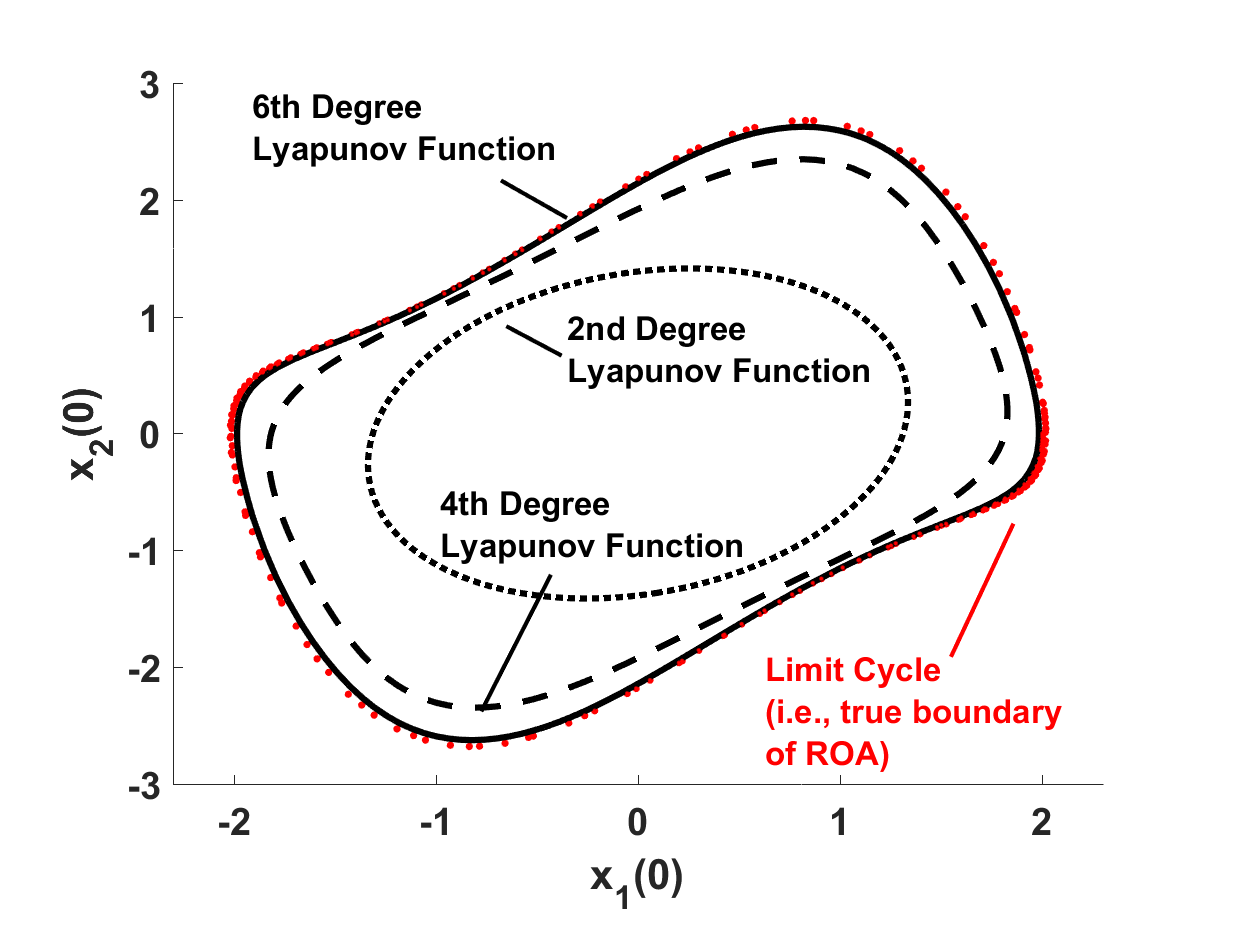
\includegraphics[width=0.85\columnwidth]{figures/my_figure.eps}
		\end{center}
	\end{itemize}
\end{frame}

%%%%%%%%%%%%%%%%%%%%%%%%%%%%
\begin{frame}[fragile,t]{Add Figures to Slides}
	\begin{itemize}
		\item PNG file (should look a little blurrier than the eps version)
		\begin{center}
			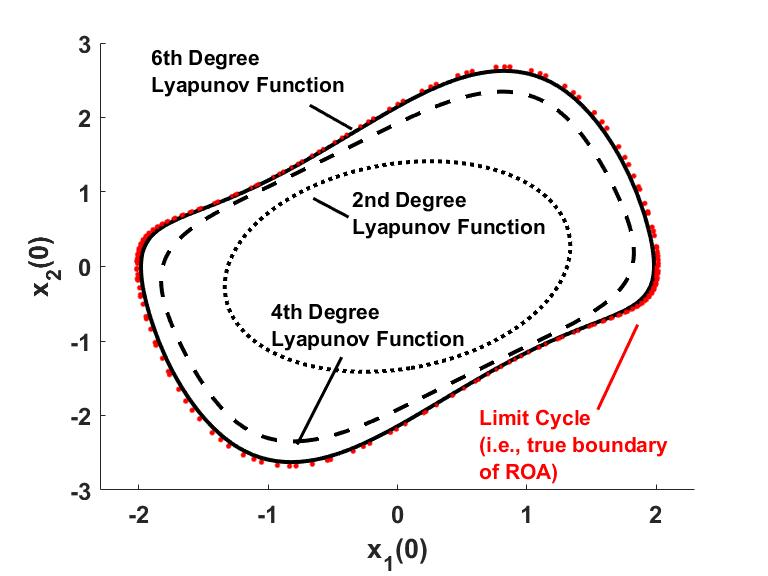
\includegraphics[width=0.85\columnwidth]{figures/my_figure.jpg}
		\end{center}
	\end{itemize}
\end{frame}


%%%%%%%%%%%%%%%%%%%%%%%%%%%%%% Slide %%%%%%%%%%%%%%%%%%%%%%%%%
%%%%%%%%%%%%%%%%%%%%%%%%%%%%
\begin{frame}[fragile,t]{Add Figures to Slides}
	\begin{itemize}
		\item Add a figure using the command
		\begin{verbatim}
			\includegraphics[picture size]{file location}
		\end{verbatim}
		\begin{itemize}
			\item \verb|[picture size]| - I use the \verb|\columnwidth| command to set width as a decimal $(0,1]$
			\begin{itemize}
				\item Ex: \verb|[width = 0.85\columnwidth]| - it scales the height of the figure to match the original aspect ratio
			\end{itemize}
			\item \verb|{file location}| - you need to match the file location and extension of the picture file
			\begin{itemize}
				\item The file location is relative to the main TeX file
				\item I typically save my figures in a subfolder labeled ``figures''
				\item Ex: \verb|{figures/my_figure.eps}|
			\end{itemize}
		\end{itemize}
	\end{itemize}
\end{frame}

%%%%%%%%%%%%%%%%%%%%%%%%%%%%
\begin{frame}[fragile,t]{Add Figures to Slides}
	\begin{itemize}
		\item Add a figure using the command
		\begin{verbatim}
			\includegraphics[picture size]{file location}
		\end{verbatim}
		\begin{itemize}
			\item \verb|[picture size]| - I use the \verb|\columnwidth| command to set width as a decimal $(0,1]$
			\begin{itemize}
				\item Ex: \verb|[width = 0.85\columnwidth]| - it scales the height of the figure to match the original aspect ratio
			\end{itemize}
			\item \verb|{file location}| - you need to match the file location and extension of the picture file
			\begin{itemize}
				\item The file location is relative to the main TeX file
				\item I typically save my figures in a subfolder labeled ``figures''
				\item Ex: \verb|{figures/my_figure.eps}|
			\end{itemize}
		\end{itemize}
		\item When appropriate, can center the figure (height and width) using
		{\small
		\begin{lstlisting}
\begin{center}
	\includegraphics[picture size]{file location}
\end{center}
		\end{lstlisting}
		}
	\end{itemize}
\end{frame}

%%%%%%%%%%%%%%%%%%%%%%%%%%%%
\begin{frame}[fragile,t]{Make a Figure}
	\begin{itemize}
		\item Here's the sample code to make the following figure
		{\tiny
		\begin{lstlisting}
\begin{center}
	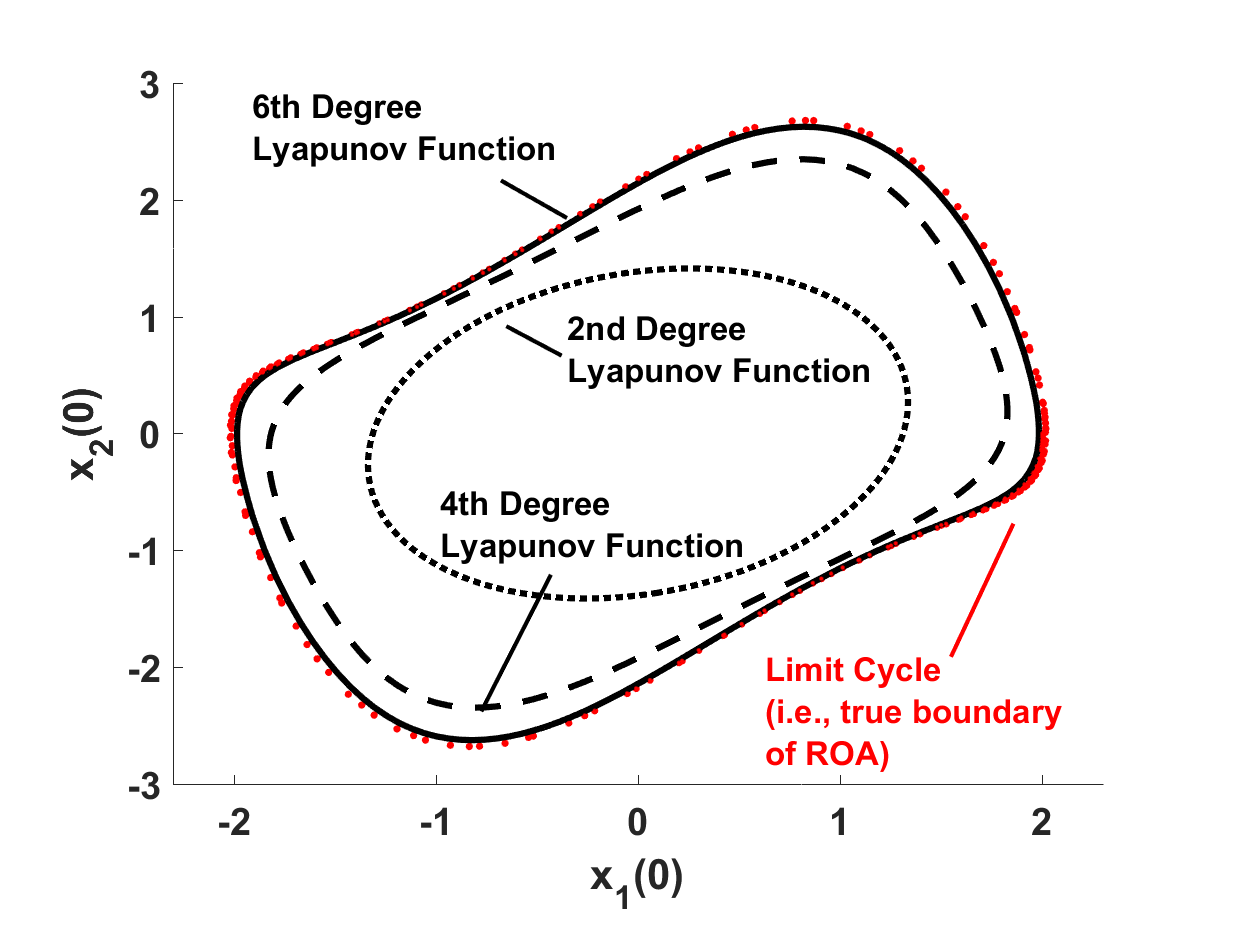
\includegraphics[width=0.65\columnwidth]{figures/my_figure.eps}
\end{center}
		\end{lstlisting}
		}
\vspace{-12pt} %removes white space between (opposite of positive values in vspace)
		\begin{center}
			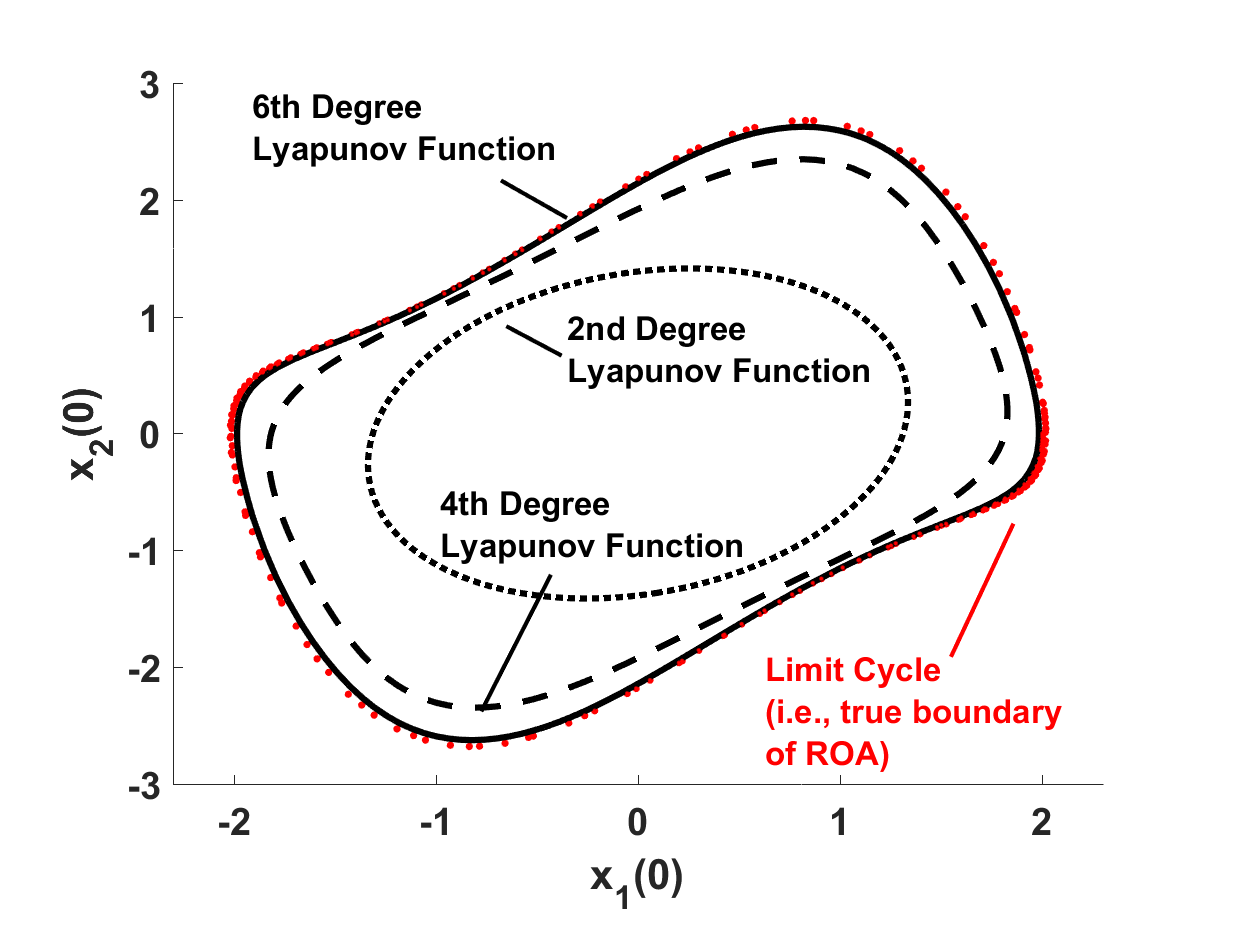
\includegraphics[width=0.65\columnwidth]{figures/my_figure.eps}
		\end{center}
		\item Note that you can nest the figure within ordered lists too
	\end{itemize}
\end{frame}


%%%%%%%%%%%%%%%%%%%%%%%%%%%%%% Slide %%%%%%%%%%%%%%%%%%%%%%%%%%
%%%%%%%%%%%%%%%%%%%%%%%%%%%%
\begin{frame}[fragile,t]{Multiple Figures}
	\begin{itemize}
		\item If you want to make multiple figures side-by-side, you can just set the sum of the figures' column widths to be $\leq 1.0$
		{\tiny
		\begin{lstlisting}
\begin{center}
	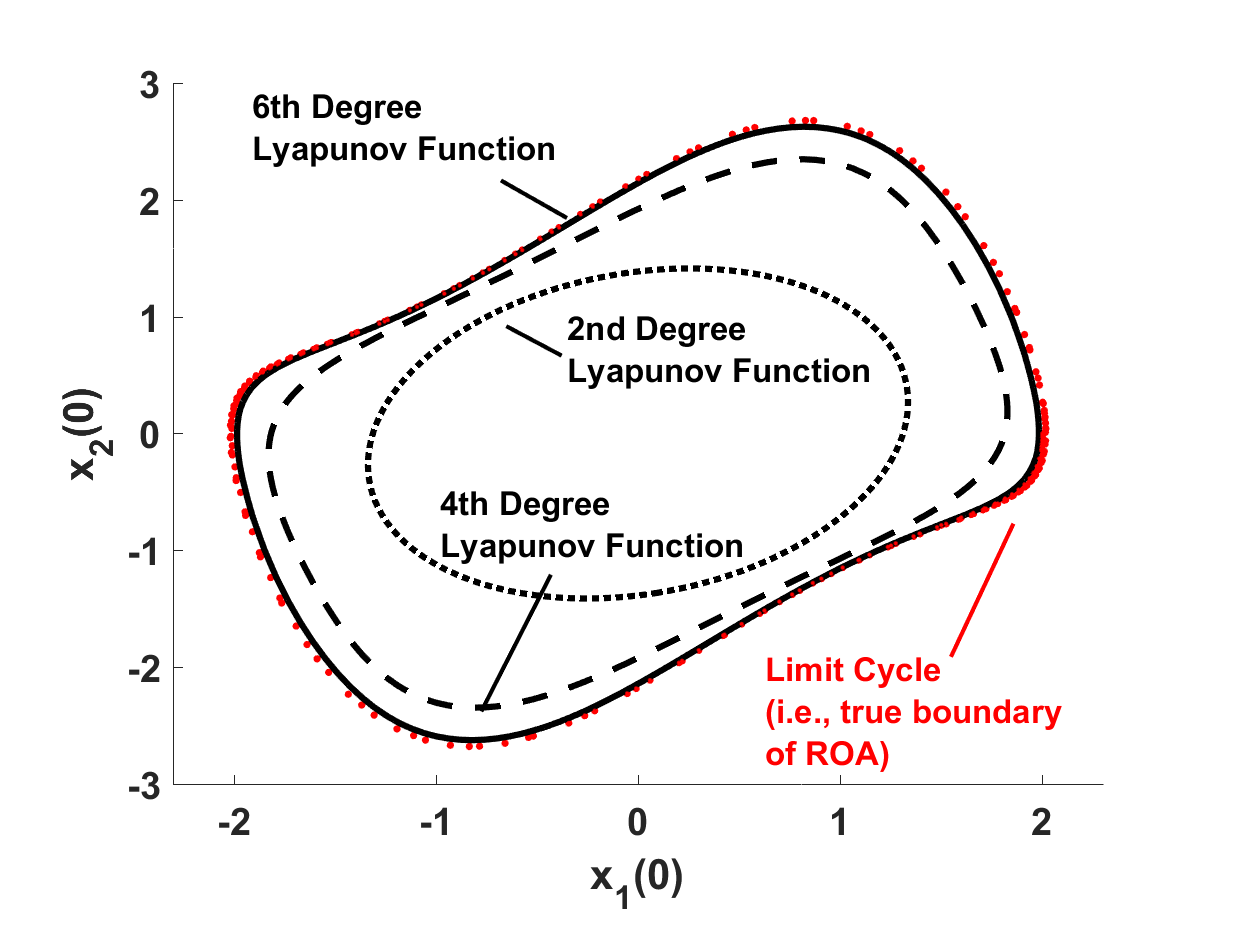
\includegraphics[width=0.35\columnwidth]{figures/my_figure.eps}
	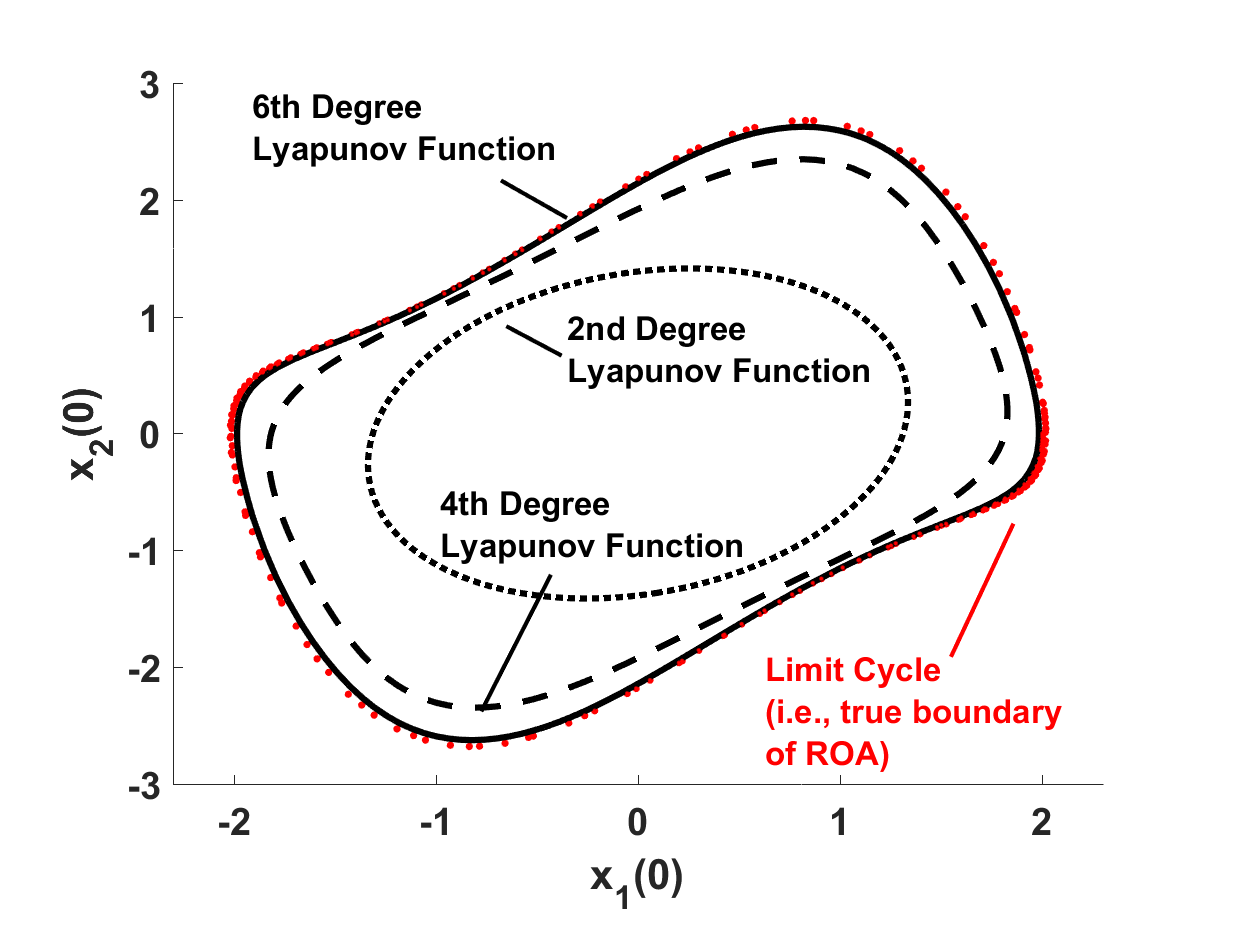
\includegraphics[width=0.45\columnwidth]{figures/my_figure.eps}
	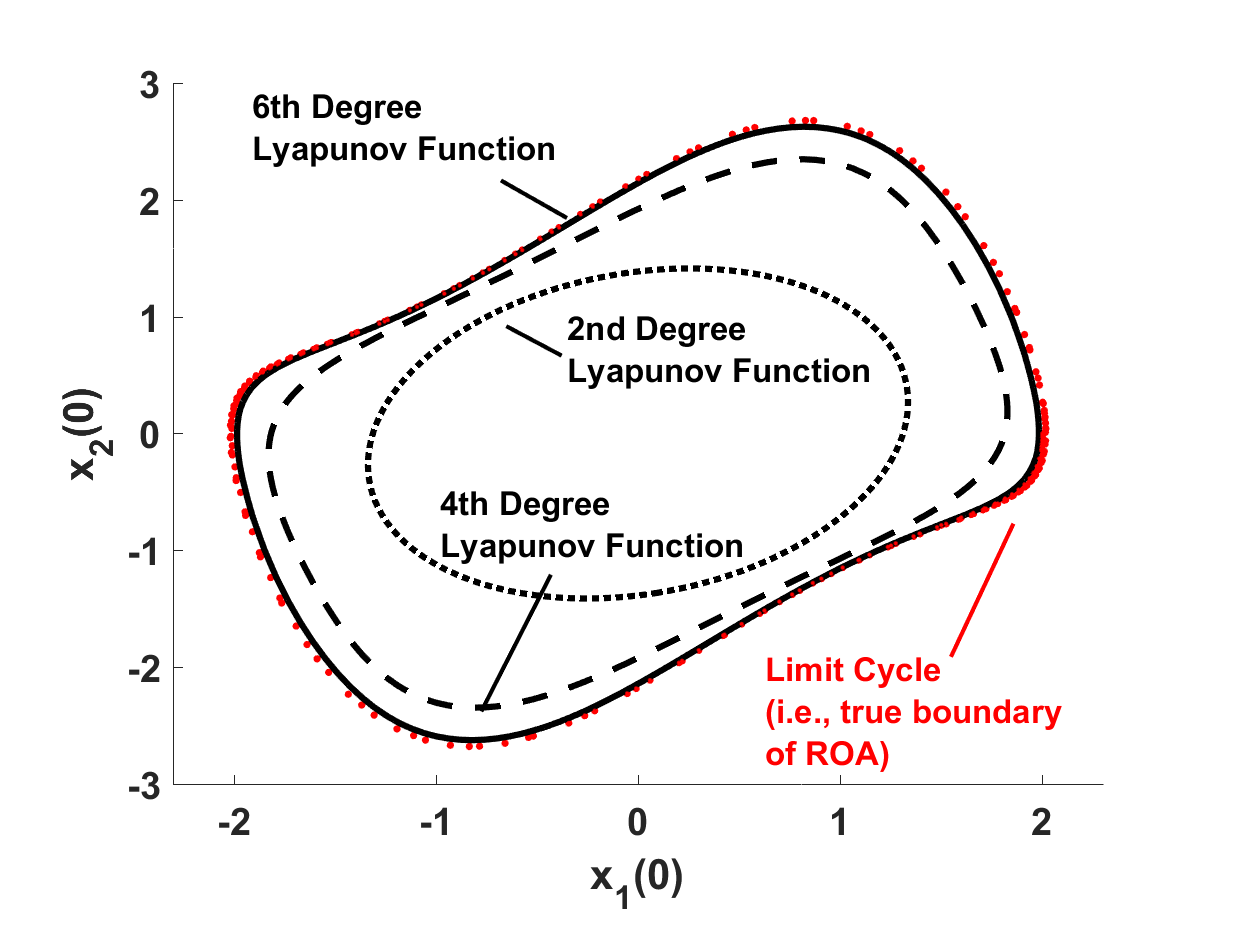
\includegraphics[width=0.15\columnwidth]{figures/my_figure.eps}
\end{center}
		\end{lstlisting}
		}
		\begin{center}
			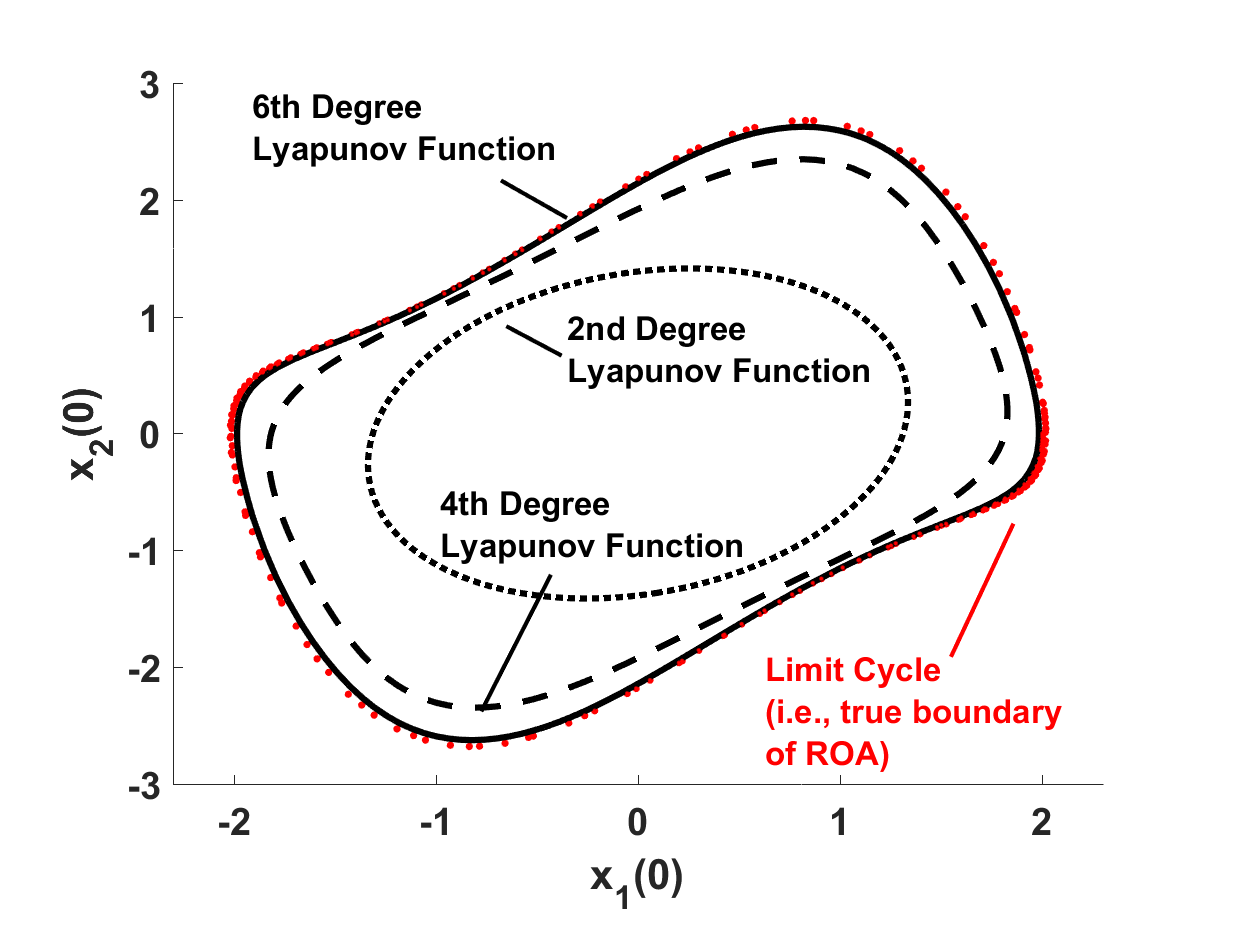
\includegraphics[width=0.35\columnwidth]{figures/my_figure.eps}
			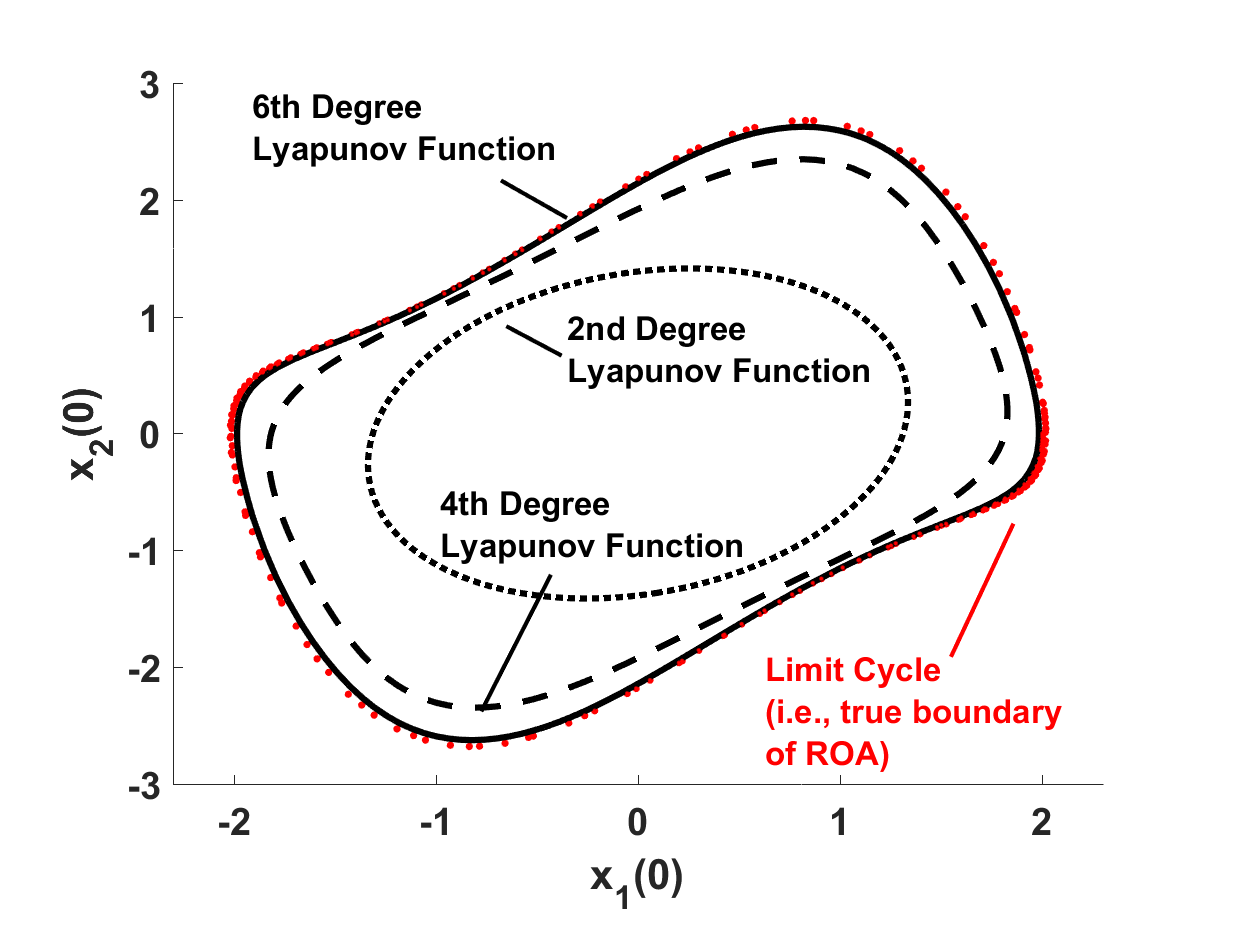
\includegraphics[width=0.45\columnwidth]{figures/my_figure.eps}
			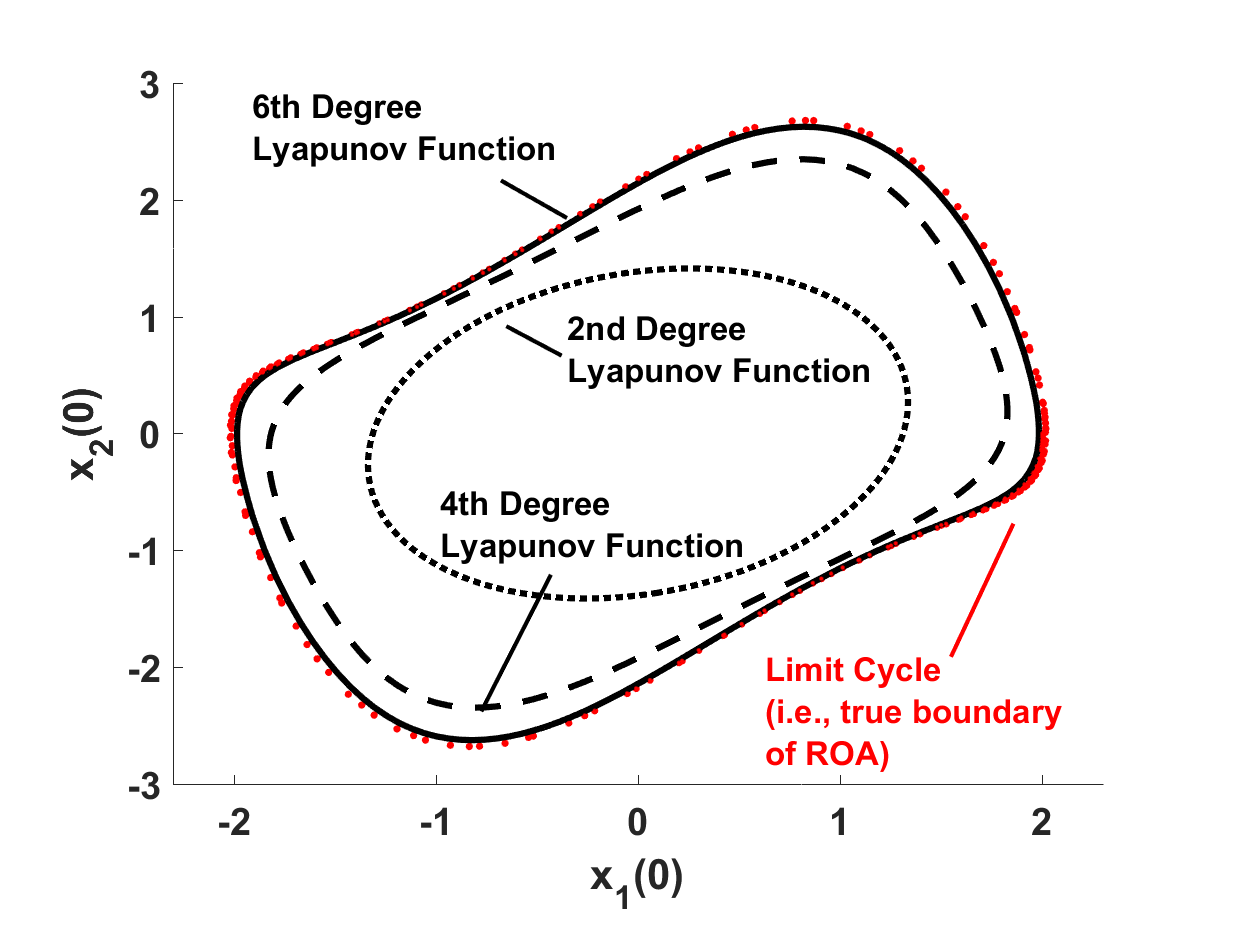
\includegraphics[width=0.15\columnwidth]{figures/my_figure.eps}
		\end{center}
		\item If the sum is $> 1.0$ then it will stack them vertically
	\end{itemize}
\end{frame}
 %Don't look at this until you've already gone through the presentation
%%%%%%%%%%%%%%%%%%%%%%%%%%%%%% Slide %%%%%%%%%%%%%%%%%%%%%%%%%%
\subsection{Columns}
%%%%%%%%%%%%%%%%%%%%%%%%%%%%
\begin{frame}[fragile,t]{Making Columns}
	\begin{itemize}
		\item Sometimes columns are easier for side-by-side text and figures
	\end{itemize}
\vspace{0.2in}
	\begin{columns}
		\begin{column}{0.49\textwidth}
		\begin{itemize}
			\item Example: text next to a picture
			\item See how I can use ordered lists just like I did before?
			\begin{itemize}
				\item All the same formatting rules still apply within a column
			\end{itemize}
			\item I could have also put the figure on the left and text on the right
		\end{itemize}
		\end{column}
		\begin{column}{0.49\textwidth}
		\centering
		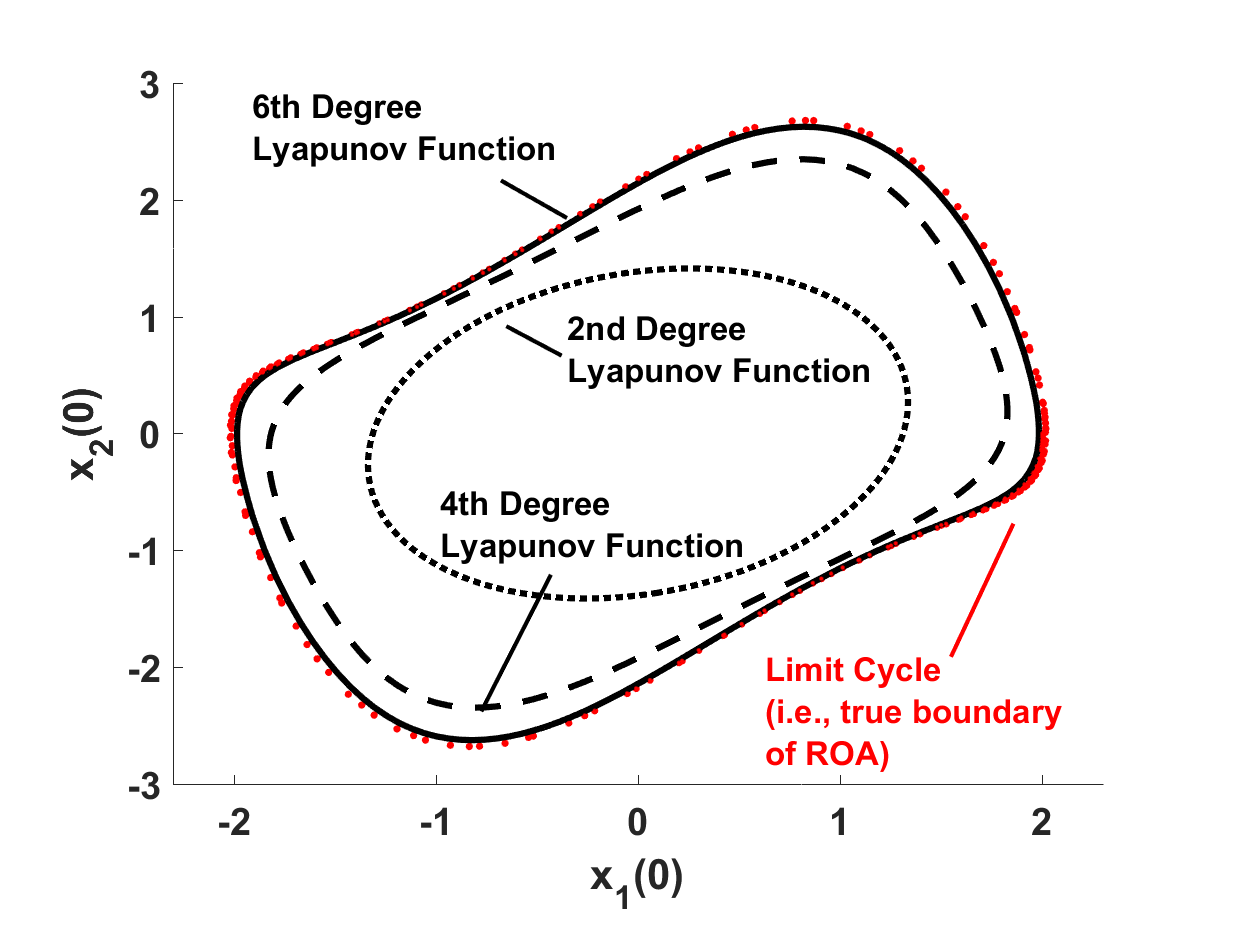
\includegraphics[width=0.9\columnwidth]{figures/my_figure.eps} 
		\end{column}
	\end{columns}
\end{frame}

%%%%%%%%%%%%%%%%%%%%%%%%%%%%
\begin{frame}[fragile,t]{Making Columns}
	\begin{itemize}
		\item Sometimes columns are easier for side-by-side text and figures
\vspace{0.2in}
		\item Or put two figures next to each other
		\begin{itemize}
			\item And add a caption
		\end{itemize}
	\end{itemize}
\vspace{0.2in}
	\begin{columns}
		\begin{column}{0.49\textwidth}
		\centering
		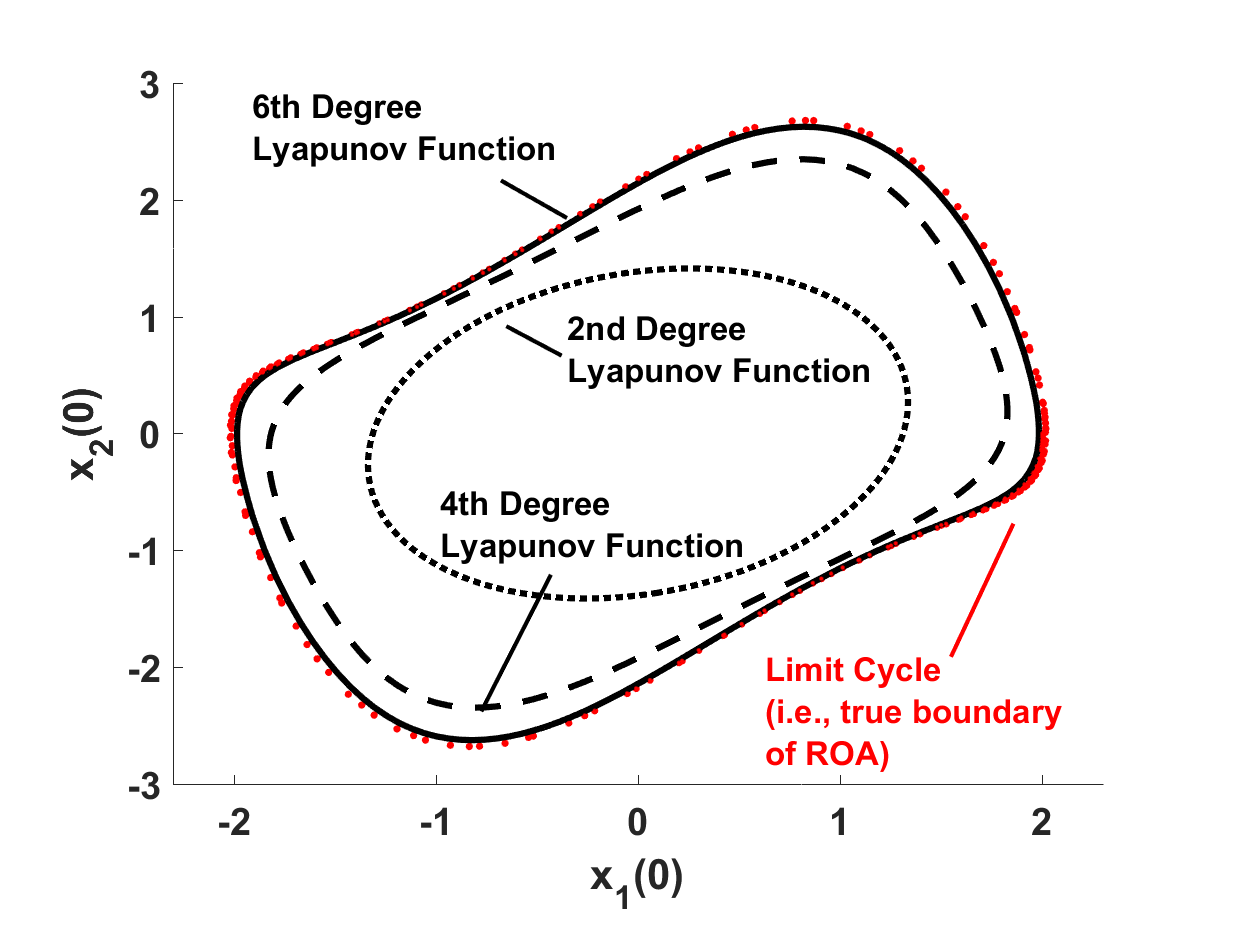
\includegraphics[width=0.9\columnwidth]{figures/my_figure.eps} 
		\\ a) caption one
		\end{column}
		\begin{column}{0.49\textwidth}
		\centering
		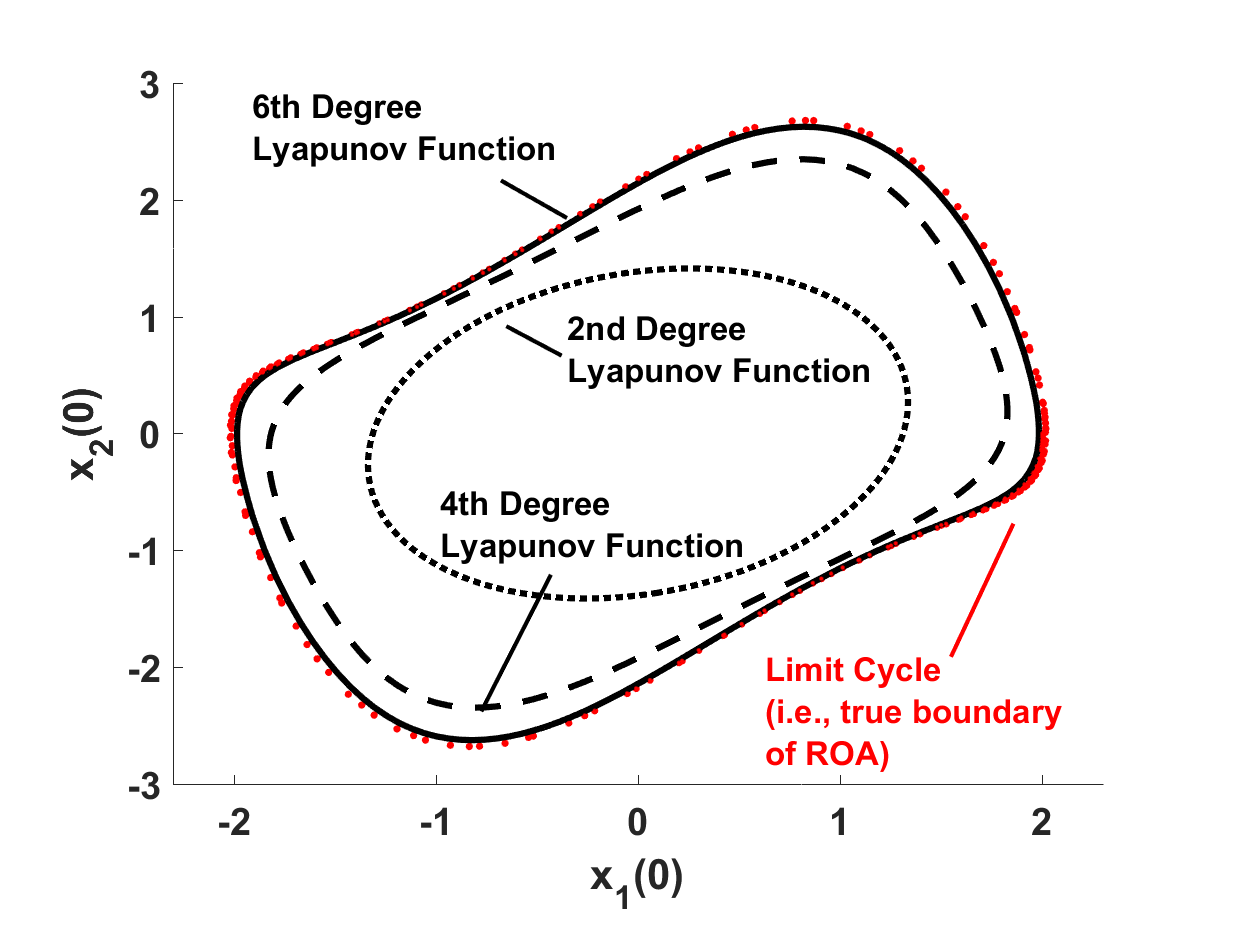
\includegraphics[width=0.9\columnwidth]{figures/my_figure.eps} 
		\\ b) caption two
		\end{column}
	\end{columns}
\end{frame}


%%%%%%%%%%%%%%%%%%%%%%%%%%%%%% Slide %%%%%%%%%%%%%%%%%%%%%%%%%%
%%%%%%%%%%%%%%%%%%%%%%%%%%%%
\begin{frame}[fragile,t]{Making Columns}
	\begin{itemize}
		\item Here's the sample code to make two columns	
{\small
	\begin{lstlisting}
\begin{columns}
	\begin{column}{0.49\textwidth}
		Add some text here
	\end{column}
	\begin{column}{0.49\textwidth}
		Add a figure here
	\end{column}
\end{columns}
	\end{lstlisting}
}
	\end{itemize}
\end{frame}

%%%%%%%%%%%%%%%%%%%%%%%%%%%%
\begin{frame}[fragile,t]{Making Columns}
	\begin{itemize}
		\item Here's the sample code to make two columns
{\small
	\begin{lstlisting}
\begin{columns}
	\begin{column}{0.49\textwidth}
		Add some text here
	\end{column}
	\begin{column}{0.49\textwidth}
		Add a figure here
	\end{column}
\end{columns}
	\end{lstlisting}
}
	\begin{itemize}
		\item Including an ordered (bulleted) list
{\small
	\begin{lstlisting}
\begin{column}{0.49\textwidth}
	\begin{itemize}
		\item Add some text here
	\end{itemize}
\end{column}
	\end{lstlisting}
}
	\end{itemize}
	\end{itemize}
\end{frame}

%%%%%%%%%%%%%%%%%%%%%%%%%%%%
\begin{frame}[fragile,t]{Making Columns}
	\begin{itemize}
		\item Here's the sample code to make two columns
{\small
	\begin{lstlisting}
\begin{columns}
	\begin{column}{0.49\textwidth}
		Add some text here
	\end{column}
	\begin{column}{0.49\textwidth}
		Add a figure here
	\end{column}
\end{columns}
	\end{lstlisting}
}
	\begin{itemize}
		\item Including a figure
{\small
	\begin{lstlisting}
\begin{column}{0.49\textwidth}
	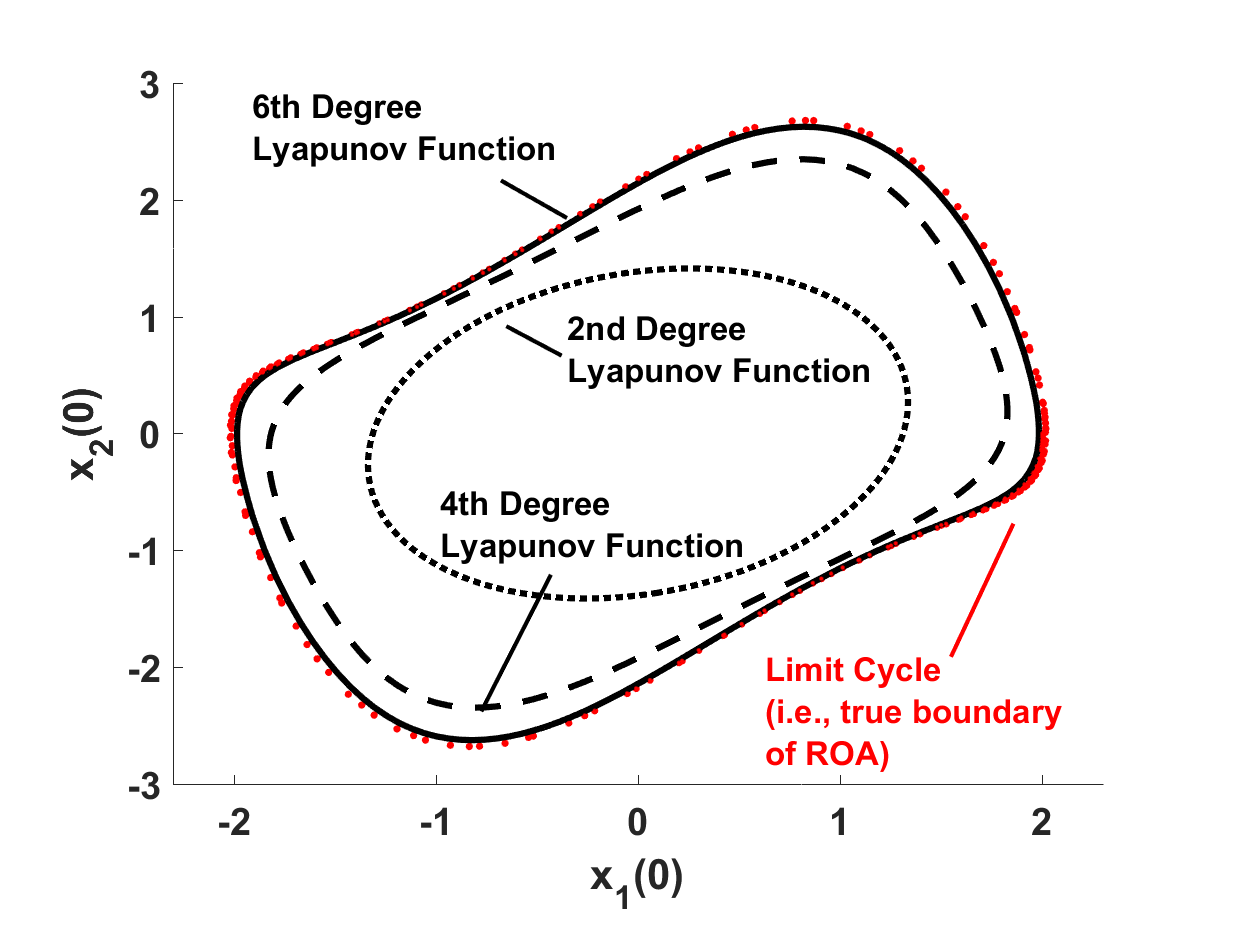
\includegraphics[width=0.9\columnwidth]{figures/my_figure.eps} 
\end{column}
	\end{lstlisting}
}
	\end{itemize}
	\end{itemize}
\end{frame} %Don't look at this until you've already gone through the presentation


%%%%%%%%%%%%%%%%%%%%%%%%%%%%%%% Slide %%%%%%%%%%%%%%%5%%%%%%%%%%
%%%%%%%%%%%%%%%%%%%%
\begin{frame}[t]{Overview} %Initializes the slide - the part within {xyz} is the title displayed at the top
	\begin{itemize} %Start a bulleted list
		\item Basic slides %Add an item in the bulleted list
		\begin{itemize} %Start a nested bulleted list
			\item Title slides %Add an item in the nested bulleted list
			\item Ordered lists
			\item Figures
			\item Columns
		\end{itemize} %End the  nested list
\vspace{0.1in} %Add extra vertical spacing
		\item Formatting %Add an item in the original bulleted list
		\begin{itemize} %Add another nested bulleted list
			\item Headers, footers, sections
			\item References and citations
			\item Overlays and pauses
		\end{itemize}
\vspace{0.1in}
		\item Misc things
		\begin{itemize}
			\item Input files
			\item Math equations/symbols
			\item Pop-up text boxes
			\item Movies
		\end{itemize}
	\end{itemize}
\end{frame}


%-----------------------------------------------------------------------------------------------------------------------------------------------%
%%%%% Once you're comfortable with the basic steps, you can start looking at the source code in these TeX files
% Formatting things
\section{Formatting Things}
%%%%%%%%%%%%%%%%%%%%%%%%%%%%%% Slide %%%%%%%%%%%%%%%%%%%%%%%%%%
\subsection{Headers and Footers}
%%%%%%%%%%%%%%%%%%%%%%%%%%%%
\begin{frame}[fragile,t]{Adding Headers} %Note that I'm throwing in a term ``fragile'' alongside the starndard ``[t]''.  You won't need to include this unless you're doing fancier formatting like I am doing with ``\verb''
	\begin{itemize}
		\item Look at the top of the slide - see the headers?
\vspace{0.2in} %adds a vertical space between the next line
		\item These can be controlled using \verb|\section{Add section}| and \verb|\subsection{Add subsection}|
\vspace{0.2in} %adds a vertical space between the next line
		\item Use the following code to change the headers
	\end{itemize}
\end{frame}

%%%%%%%%%%%%%%%%%%%%%%%%%%%%
\begin{frame}[fragile,t]{Adding Headers} 
	\begin{lstlisting} 
\section{This controls section name}
\subsection{This controls subsection name}
\begin{frame}[t]{Example Slide 1}
	Add your text here
\end{frame }

\subsection{Change subsection name}
\begin{frame}[t]{Example Slide 2}
	Notice the section name didn't change
\end{frame }
	\end{lstlisting} %End
\end{frame}

%%%%%%%%%%%%%%%%%%%%%%%%%%%%
\section{This controls section name}
\subsection{This controls subsection name}
\begin{frame}[t]{Example Slide 1} %Example slides
	Add your text here
\end{frame}

\subsection{Change subsection name}
\begin{frame}[t]{Example Slide 2}
	Notice the section name didn't change
\end{frame}
\section{Formatting Things} %Reset section
\subsection{Headers and Footers} %Reset subsection


%%%%%%%%%%%%%%%%%%%%%%%%%%%%%% Slide %%%%%%%%%%%%%%%%%%%%%%%%%%
%%%%%%%%%%%%%%%%%%%%%%%%%%%%
\begin{frame}[fragile,t]{Changing Frame Number}
	\begin{itemize}
		\item By default, the frame number increases with each new frame
\vspace{0.2in}
		\item You can manually change the frame counter by positive or negative integers
		\begin{itemize}
			\item Useful if you want to ``freeze'' slides or iteratively display things
		\end{itemize}
		\begin{lstlisting}
\addtocounter{framenumber}{-1}
\begin{frame}[t]{New slide}
	Notice the frame number didn't change
\end{frame }
		\end{lstlisting}
	\end{itemize}
\end{frame}
%%%%
\addtocounter{framenumber}{-1}
\begin{frame}[t]{New slide}
	Notice the frame number didn't change (bottom right corner)
\end{frame}
%%%%%%%%%%%%%%%%%%%%%%%%%%%%%% Slide %%%%%%%%%%%%%%%%%%%%%%%%%%
\subsection{Handling References}
%%%%%%%%%%%%%%%%%%%%%%%%%%%%
\begin{frame}[fragile,t]{Adding References} 
	\begin{itemize}
		\item Two things needed for references
		\begin{enumerate}
			\item Add a citation in the text
			\item Link to a bibliography (.bibtex) file
		\end{enumerate}
	\end{itemize}
	\begin{enumerate}
		\item Add a citation in the text
		\begin{itemize}
			\item Multiple commands to add citations
\vspace{0.1in}
			\item The \verb|\cite{bibtexkey}| command adds a number: blah blah blah\cite{liu2016learning}
			\item The \verb|\citet{bibtexkey}| command adds a name too: blah blah blah (\citet{Omidshafiei16_HBNIarxiv})
			\item You can do other options, but you'll have to go through and add some new packages
			\item You can also do multiple in a single call - \verb|\cite{bibtexkey2,bibtexkey3}|: blah blah blah \cite{Omidshafiei16_HBNIarxiv,Quindlen16_ACC}
		\end{itemize}
	\end{enumerate}
\end{frame}

%%%%%%%%%%%%%%%%%%%%%%%%%%%%
\begin{frame}[fragile,t]{Adding References} 
	\begin{enumerate}
		\item Add a citation in the text
		\item Link to a bibliography (.bibtex) file
		\begin{itemize}
			\item Add a bibliography file to the document - I keep mine in a ``references'' subfolder or something similar
			\begin{itemize}
				\item Here I used the bibtex file ``ACL\_publications.bib''
			\end{itemize}
			\item Also need to specify a bibliography style, ex: ``unstr''
\vspace{0.1in}
			\item I usually place the link to the bibliography file at the very end of the document
\vspace{0.2in}
			\item Here's the sample code used at the end of this presentation
			\begin{lstlisting}
\begin{frame}[allowframebreaks]{References}
\bibliographystyle{unsrt}
\bibliography{references/ACL_publications}
\end{frame }
\end{document}
			\end{lstlisting}
		\end{itemize}
	\end{enumerate}
\end{frame}

%Bibliography
\begin{frame}[allowframebreaks]{References}
\bibliographystyle{unsrt}
\bibliography{references/ACL_publications}
\end{frame}

%%%%%%%%%%%%%%%%%%%%%%%%%%%%%% Slide %%%%%%%%%%%%%%%%%%%%%%%%%%
%%%%%%%%%%%%%%%%%%%%%%%%%%%%
\begin{frame}[t]{Making References} 
	\begin{itemize}
		\item The previous slides showed how to add citations and link to a bibliography file, but you must first create that bibliography file
		\begin{itemize}
			\item There's already some bibliography files for the lab's own paper: \\
			\url{svn://acl.mit.edu/acl/BIB_all/ACL_Publications.bib}
		\end{itemize}
\vspace{0.2in}
		\item If you want to make your own bibliography you can use software such as \href{http://www.jabref.org/}{JabRef} to organize your files more easily
\vspace{0.2in}
		\item Especially if you're putting them into the ACL-common files, use the following style for your BibTex key:
		\begin{itemize}
			\item ``Last Name\ + \ Year (last two digits) + \_ + Journal/Conference Initials''
			\item Example: ``Jack Quindlen'' + ``2016'' + ``American Control Conference'' = ``Quindlen16\_ACC''
		\end{itemize}
	\end{itemize}
\end{frame}
%%%%%%%%%%%%%%%%%%%%%%%%%%%%%% Slide %%%%%%%%%%%%%%%%%%%%%%%%%%
\subsection{Overlays}
%%%%%%%%%%%%%%%%%%%%%%%%%%%%
\begin{frame}[fragile,t]{Adding Overlays} 
	\begin{itemize}
		\item Here's how you can overlay text
\pause
		\item So that you can leave it temporarily blurred out
\pause
		\item One of the easiest ways to do so is with the \verb|\pause| command
		\begin{itemize}
			\item Here's the code I just used:
			\begin{lstlisting}
\item Here's how you can overlay text
\pause
\item So that you can leave it temporarily blurred out
\pause
\item One of the easiest ways to do so is with the
			\end{lstlisting}
\pause
			\item Each \verb|\pause| command hides the text that follows and they stack upon each other
		\end{itemize}
	\end{itemize}
\end{frame}


%%%%%%%%%%%%%%%%%%%%%%%%%%%%%% Slide %%%%%%%%%%%%%%%%%%%%%%%%%%
%%%%%%%%%%%%%%%%%%%%%%%%%%%%
\begin{frame}[fragile,t]{Adding Overlays} 
	\begin{itemize}
		\item<1-4> Another way to do it is within the itemize framework
\vspace{0.1in}
		\item<2-> When you command \verb|\item|, you can specify in which frame(s) the text will be displayed
		\begin{itemize}
			\item You just have to add ``$<$frame number(s)$>$'' immediately after \verb|\item|
			\item Example: \verb|\item<2>| will only display the text in the second frame
			\item<3-> You can also make them stay visible using a hyphen
			\item<3-> Example: \verb|\item<2->| will display the text in the second and all subsequent frames
		\end{itemize}
\vspace{0.1in}
		\item<4-> You can also use that to make text disappear
		\begin{itemize}
			\item<5-> See what just happened with the first bullet point?
			\item<5-> I used \verb|\item<1-4>| to make it disappear after the fourth frame
		\end{itemize}
	\end{itemize}
\end{frame}


%%%%%%%%%%%%%%%%%%%%%%%%%%%%%% Slide %%%%%%%%%%%%%%%%%%%%%%%%%%
%%%%%%%%%%%%%%%%%%%%%%%%%%%%
\begin{frame}[fragile,t]{Adding Overlays} 
	\begin{itemize}
		\item Lastly, another simple option is to just make two copies of the same slide, one with additional material
		\begin{itemize}
			\item Can use the \verb|\addtocounter{framenumber}{-1}| command we discussed to freeze the frame counter
			\item This is particularly useful when you have figures because the previous two methods have problems
		\end{itemize}
\pause
\vspace{0.1in}
		\item You can also try more advanced commands such as \verb|\only<2->| or \verb|\visible<2->| or \verb|\uncover<2->|
		\begin{itemize}
			\item They all have their own nuances, Google it if you think you need to use them
		\end{itemize}
	\end{itemize}
\end{frame}





%%%%%%%%%%%%%%%%%%%%%%%%%%%%%%% Slide %%%%%%%%%%%%%%%5%%%%%%%%%%
%%%%%%%%%%%%%%%%%%%%
\begin{frame}[t]{Overview} %Initializes the slide - the part within {xyz} is the title displayed at the top
	\begin{itemize} %Start a bulleted list
		\item Basic slides %Add an item in the bulleted list
		\begin{itemize} %Start a nested bulleted list
			\item Title slides %Add an item in the nested bulleted list
			\item Ordered lists
			\item Figures
			\item Columns
		\end{itemize} %End the  nested list
\vspace{0.1in} %Add extra vertical spacing
		\item Formatting %Add an item in the original bulleted list
		\begin{itemize} %Add another nested bulleted list
			\item Headers, footers, sections
			\item References and citations
			\item Overlays and pauses
		\end{itemize}
\vspace{0.1in}
		\item Misc things
		\begin{itemize}
			\item Input files
			\item Math equations/symbols
			\item Pop-up text boxes
			\item Movies
		\end{itemize}
	\end{itemize}
\end{frame}


%-----------------------------------------------------------------------------------------------------------------------------------------------%
%%%%% Other stuff that to consider %%%%%%%%%%%
\section{Misc}
%%%%%%%%%%%%%%%%%%%%%%%%%%%%%%%%%%%% Slide %%%%%%%%%%%%%%%%%%%%%%%%%%%%
%%%%%%%%%%%%%%%%%%%%%%%%%%%%
\begin{frame}[fragile,t]{Spaces}
	\begin{itemize}
		\item If you want to add extra white space (or subtract some) you can use the \verb|\vspace{xyz}| and \verb|\hspace{xyx}| commands
		\begin{itemize}
			\item You can use units of ``pts'' (as in font size), ``in'' for inches, or ``cm'' for centimeters
			\item Example: \verb|\vspace{0.2in}| for $0.2$ inch or \verb|\vspace{12pt}| for 12 points
		\end{itemize}
\vspace{0.1in}
		\item \verb|\vspace{xyz}| controls the vertical spacing
		\begin{itemize}
\vspace{0.05in}
			\item Using positive values adds extra white space between lines
\vspace{-0.05in}
			\item Using negative values shrinks the white space between lines/objects
			\item You can also add ``\verb|\\|'' to the end of a line to force a new line
		\end{itemize}
\vspace{0.1in}
		\item \verb|\hspace{xyz}| controls the horizontal spacing
		\begin{itemize}
			\item \hspace{0.2in} Using positive values pushes text right
			\item \hspace{-0.25in} Using negative values pushes text left
			\item You can also add an extra spacebar using a backslash ``$\backslash$''
		\end{itemize}
	\end{itemize}
\end{frame}


%%%%%%%%%%%%%%%%%%%%%%%%%%%%%%%%%%%% Slide %%%%%%%%%%%%%%%%%%%%%%%%%%%%
%%%%%%%%%%%%%%%%%%%%%%%%%%%%
\begin{frame}[fragile,t]{Input Files}
	\begin{itemize}
		\item When dealing with large presentations, it can become difficult to use a single .tex file
		\begin{itemize}
			\item Instead use \verb|\input{filename}| to break up one file into several
		\end{itemize}
\vspace{0.1in}
		\item I use a single ``root'' file titled ``main.tex'' that calls several input files, labeled something like ``sec\_blahblahblah.tex''
		\item Nothing new is needed in the input file - no special ``begin{}'' etc - just start making frames as you would otherwise
		\item All you need is a command \verb|\input{sec_blahblahblah}| in the root folder - it will include all the frames in ``sec\_blahblahblah'' before the next set of slides
		{\tiny
		\begin{lstlisting}
\begin{frame}[t]{This is the 1st slide}
	Blah blah blah
\end{frame }
\input{sec_TenSlides} %insert the 10 slides specified by the file ``sec_TenSlides.tex''
\input{sec_FiveSlides} %insert the 5 slides specified by the file ``sec_FiveSlides.tex''
\begin{frame}[t]{This is the 17th slide}
	Blah blah blah
\end{frame }
		\end{lstlisting}
		}
	\end{itemize}
\end{frame}

%%%%%%%%%%%%%%%%%%%%%%%%%%%%
\addtocounter{framenumber}{-1}
\begin{frame}[t]{Input Files}
	\begin{center}
		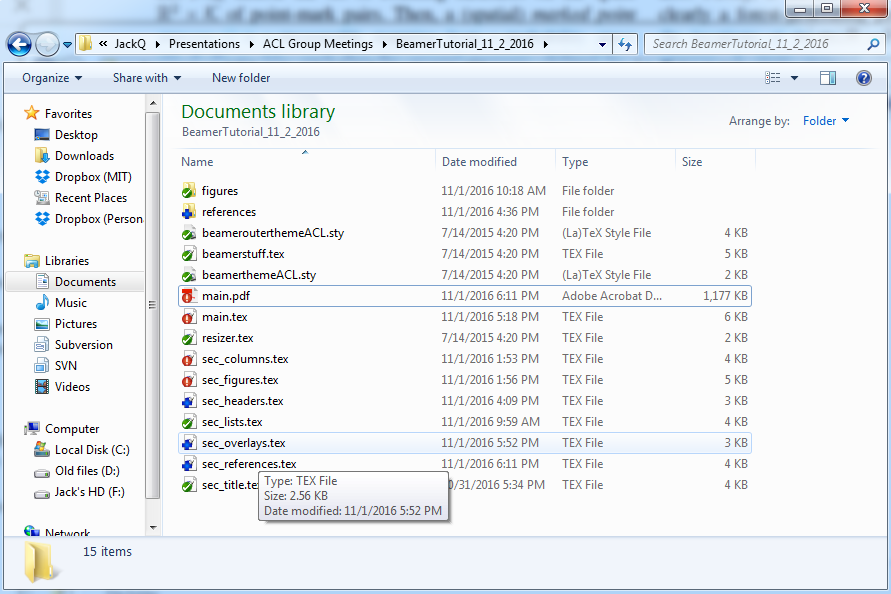
\includegraphics[width=0.95\columnwidth]{figures/folderView.png}
	\end{center}
\end{frame}


%%%%%%%%%%%%%%%%%%%%%%%%%%%%%%%%%%%% Slide %%%%%%%%%%%%%%%%%%%%%%%%%%%%
%%%%%%%%%%%%%%%%%%%%%%%%%%%%
\begin{frame}[fragile,t]{Math Equations/Symbols}
	\begin{itemize}
		\item No modifications have to be made to write mathematical equations or symbols while operating in beamer
		\begin{lstlisting}
\begin{frame}[t]{Math Equations}
	You can still add math symbols to sentences 
	by using dollar signs\\
	like this $1 + 1 = \alpha$ \\
\vspace{0.2in}
	And use equations in the same way like
	\begin{equation}
		1 + 1 = \alpha
	\end{equation}
\end{frame }
		\end{lstlisting}
		\item Check out \href{https://en.wikibooks.org/wiki/LaTeX/Mathematics}{HERE} and \href{http://www.colorado.edu/physics/phys4610/phys4610_sp15/PHYS4610_sp15/Home_files/LaTeXSymbols.pdf}{HERE} if you don't know LaTeX math
	\end{itemize}
\end{frame}


%%%%%%%%%%%%%%%%%%%%%%%%%%%%%%%%%%%% Slide %%%%%%%%%%%%%%%%%%%%%%%%%%%%
%%%%%%%%%%%%%%%%%%%%%%%%%%%%
\begin{frame}[fragile,t]{Pop-Up Text Blocks}
	\begin{itemize}
		\item You can hard code pop-up text blocks
		\begin{itemize}
			\item You'll have to include the following code immediately following the other packages at the beginning of the document		
			{\tiny
			\begin{lstlisting}
\usepackage[absolute,overlay]{textpos} 
\newenvironment{myfootnote}[3]{%
\begin{textblock*}{#3}(#1,#2) 
\tiny\begingroup\color{blue!50!black}}{\endgroup\end{textblock*}}
			\end{lstlisting}
			}
			\item Then you'll create a textbox using
			{\tiny
			\begin{lstlisting}
\only<2->{
\begin{textblock*}{0.99\textwidth}(0.05\textwidth,37ex) 
	\begin{block}{Textbox title}
		Whatever you say in the textbox
	\end{block}
\end{textblock*}
}
			\end{lstlisting}
			}
			\begin{itemize}
				\item The \verb|\only<2->| command makes the textbox only popup in the second frame
				\item The line \verb|\begin{textblock*}{0.99\textwidth}(0.05\textwidth,37ex)| sets \{width of textblock\}(distance from left of page, distance from top of page)
			\end{itemize}
		\end{itemize}
	\end{itemize}
	\only<2->{
	\begin{textblock*}{0.99\textwidth}(0.05\textwidth,10ex) 
		\begin{block}{Textbox title}
			\begin{itemize}
				\item It does something like this!
				\item Notice that I can do all the other commands (like bulleted lists) in here too!
			\end{itemize}
		\end{block}
	\end{textblock*}
	}
\end{frame}
	
%%%%%%%%%%%%%%%%%%%%%%%%%%%%%%%%%%%% Slide %%%%%%%%%%%%%%%%%%%%%%%%%%%%
\subsection{Adding Movies}
%%%%%%%%%%%%%%%%%%%%%%%%%%%%
\begin{frame}[t]{Adding Movies}
	\begin{itemize}
		\item You can also add movies to beamer presentations
		\begin{enumerate}
			\item Embed Youtube links
			\item Embed local videos stored on your hard drive
		\end{enumerate}
\vspace{0.2in}
		\item I took these slides from my earlier presentation
		\begin{itemize}
			\item I didn't include local videos
			\item You can find that complete presentation here \url{svn://acl.mit.edu/acl/ACL_Beamer_Template/movie_making.tex}
		\end{itemize}
	\end{itemize}
\end{frame}

%%%%%%%%%%%%%%%%%%%%%%%%%%%%%%%%%%%%% New slide
\begin{frame}[t]{Notes}
	\begin{itemize}
		\item \textbf{Intro}: you should use this as a template for embedding videos.  Copy and paste it into your code as necessary
\vspace{12pt}
		\item I've tested this on both Windows and Ubuntu
		\begin{itemize}
			\item Depending on your compiler, you might not be able to see the videos in your compiler's display, but you can view it when you open it in Adobe Reader/Acrobat
		\end{itemize}
\vspace{12pt}
		\item \textbf{However}, I have not been able to get the videos to display properly in Ubuntu
		\begin{itemize}
			\item It correctly compiles - the videos are embedded, but the presentation software can't display it
			\item I've tried Adobe Reader 9, Okular in Ubuntu but have not been able to get videos to display properly
			\item Feel free to edit this if you do get it to work!
		\end{itemize}
	\end{itemize}
\end{frame}

%%%%%%%%%%%%%%%%%%%%%%%%%%%%%%%%%%%%% New slide
\begin{frame}[t]{Notes}
	\begin{itemize}
		\item Two ways to embed videos in your presentation:
		\begin{enumerate}
			\item Youtube (or whatever else) links embedded in the player
			\item Local files on your hard drive
		\end{enumerate}
\vspace{12pt}
		\item This uses the media9 package.  You have to make sure it's added - see line 18 of the TeX code
\vspace{24pt}
		\item Start with Youtube videos
	\end{itemize}
\end{frame}


%%%%%%%%%%%%%%%%%%%%%%%%%%%%%%%%% New slide - THIS IS A YOUTUBE LINK EXAMPLE
\begin{frame}[t]{Youtube Video}
	\begin{itemize}
		\item This is the baseline example
	\end{itemize}
	\begin{figure}
	\centering
\includemedia[
	    width=0.9\paperwidth,height=0.5\linewidth,
	    activate=pageopen, %Load the video (but you'll have to click the button to start)
	    flashvars={autoPlay=true}
	        ]{}{https://www.youtube.com/v/opsmd5yuBF0} %URL of video
        \end{figure}
\end{frame}

%%%%%%%%%%%%%%%%%%%% New slide - THIS IS A YOUTUBE LINK EXAMPLE - BETTER BECAUSE IT REMOVES TITLEBAR AND WHATNOT
\begin{frame}[t]{Youtube Video}
	\begin{itemize}
		\item This removes the title bar from the top of the video
	\end{itemize}
	\begin{figure}
	\centering
\includemedia[
	    width=0.9\paperwidth,height=0.5\linewidth,
	    activate=pageopen, %Load the video (but you'll have to click the button to start)
	    flashvars={modestbranding=1 % no YT logo in control bar
        		&autohide=1 % controlbar autohide activated
        		&showinfo=0 % no title and other info before start
        		&rel=0 % no related videos after end}
        		}
	        ]{}{https://www.youtube.com/v/opsmd5yuBF0?rel=0} %URL of video (I'm not sure if you need to put the ``?rel=0'' at the end of the URL or in the ``flashvars'' command.  I just put it in both to be safe
        \end{figure}
        %{https://www.youtube.com/v/opsmd5yuBF0}
\end{frame}

%%%%%%%%%%%%%%%%%%%%%%%%%%%%%%%%%%% New slide
\begin{frame}[t]{Youtube Video}
	\begin{itemize}
		\item \textbf{Important notes:}
		\begin{itemize}
			\item If you copy the URL straight from your browser, the link will look like: \url{https://www.youtube.com/watch?v=opsmd5yuBF0}
\vspace{6pt}
			\item But you can't use that link - you need to replace ``.../watch?v=...'' with ``.../v/...''			\vspace{6pt}
			\item When you copy your link into the beamer code, that same link will now look like:
				\url{https://www.youtube.com/v/opsmd5yuBF0}
\vspace{6pt}
			\item You can also add ``rel=0'' to prevent the related videos from showing up at the end.  New url would look like:
			\url{https://www.youtube.com/v/opsmd5yuBF0?rel=0}
		\end{itemize}
	\end{itemize}
\end{frame}

%%%%%%%%%
\frame{\titlepage} %Redisplay the title page (such as at the end of the presentation)


%-----------------------------------------------------------------------------------------------------------------------------------------------%
%Bibliography
\begin{frame}[allowframebreaks]{References}
\bibliographystyle{unsrt}
\bibliography{references/ACL_publications}
\end{frame}
\end{document} %Need this to end the document
